%Definition des informations du document
\documentclass[a4paper,12pt]{article}
\title{Projet de programmation - QR code dynamique\\Cahier des besoins}
\author{Theo El Houlali, Alexis Henquinet, Thomas Barillot,\\Bourhanoudine Mamodhoussen, Thierno Amadou Diallo, Dimitri Didier
}

%Définition des marges etc..
\setlength{\hoffset}{-18pt}        
\setlength{\oddsidemargin}{9pt} % Marge gauche sur pages impaires
\setlength{\evensidemargin}{9pt} % Marge gauche sur pages paires
\setlength{\marginparwidth}{54pt} % Largeur de note dans la marge
\setlength{\textwidth}{481pt} % Largeur de la zone de texte (17cm)
\setlength{\voffset}{-18pt} % Bon pour DOS
\setlength{\marginparsep}{7pt} % Séparation de la marge
\setlength{\topmargin}{0pt} % Pas de marge en haut
\setlength{\headheight}{0pt} % Haut de page
\setlength{\headsep}{0pt} % Entre le haut de page et le texte
\setlength{\footskip}{27pt} % Bas de page + séparation
\setlength{\textheight}{708pt} % Hauteur de la zone de texte (25cm)

%Import des différents package
\usepackage{graphicx}
\usepackage[T1]{fontenc}
\usepackage[utf8]{inputenc}
\usepackage[francais]{babel}
\usepackage{amsfonts,amsmath,amssymb}
\usepackage{fancyhdr}
\usepackage{stmaryrd}
\usepackage{eqnarray}
\usepackage{tikz}
\usepackage[hidelinks]{hyperref}
\usepackage[many]{tcolorbox}
\usepackage{booktabs}
\usepackage{listings}

\usepackage{float}
\usepackage{longtable}

%Réglages de l'en-tête et du pied de page
\renewcommand{\headrulewidth}{0.5pt}
\renewcommand{\footrulewidth}{0.5pt}

%Définition des commandes et des environnements
\newcommand\saut[1]{\vspace{#1\baselineskip}}

\newcommand\Land[0]{\bigwedge}
\newcommand\Lor[0]{\bigvee}
\newcommand\prive[0]{\setminus}


\newtcolorbox{theoreme_bis}[1]{
    tikznode boxed title,
    enhanced,
    arc=0mm,
    interior style={white},
    attach boxed title to top center= {yshift=-\tcboxedtitleheight/2},
    colbacktitle=white,coltitle=black,
    boxed title style={size=normal,colframe=white,boxrule=0pt},
    title={#1}}
    
\newenvironment{encadre}[1]
{
\begin{theoreme_bis}{#1}
}
{
\end{theoreme_bis}
}

%contenu du document

\begin{document}


\begin{titlepage}
  \begin{sffamily}
  \begin{center}
	
\includegraphics[scale=0.2]{universite.jpg}~\\[1cm]

    \textsc{\Large Projet de programmation - QR code Dynamique }\\[1.5cm]
    Sujet proposé par : Serge Chaumette\\
    Chargé de TD : Boris Mansencal

    % Titre
    \rule{1\linewidth}{2pt}
     \\[1cm]
    { \huge \bfseries Cahier des besoins\\[1cm] }
    \rule{1\linewidth}{2pt}
    \\[3cm]
    
\includegraphics[scale=1]{qr.png}
    \\[1cm]

    % Membres du groupe
   \vfill
      \begin{center}
        Theo El Houlali \hspace*{3.1cm} Thierno Amadou Diallo \hspace*{1.1cm} Thomas Barillot\\
        Bourhanoudine Mamodhoussen \hspace*{1cm} Alexis Henquinet \hspace*{2cm} Dimitri Didier
      \end{center}
 
    % Bas de la page
 
  \end{center}
  \end{sffamily}
\end{titlepage}

\newpage

%\renewcommand{\contentsname}{Sommaire}
\tableofcontents
\newpage

\section{Introduction}


L'objectif de ce projet est de mettre en œuvre un système de QR codes dynamiques, c'est-à-dire que son contenu évolue au cours du temps. Cela permet par exemple de donner au QR code une durée de vie limitée et/ou de modifier son contenu suivant des paramètres.\\

\noindent Ces paramètres peuvent être l'heure de la journée, un jour de la semaine, mais on peut aussi imaginer des paramètres non-temporels comme la météo ou le nombre de voiture sur un parking (la génération et/ou l'obtention de ces informations ne font pas partie du sujet).\\

\noindent Un exemple d'utilisation pourrait être : un QR code dynamique affiché sur le site web d'une entreprise, qui une fois scanné déclenche un appel téléphonique vers un numéro de garde qui varie selon les plages horaires.\\

\noindent Ce concept de dynamisme devra être paramétrable au moyen de \textbf{plugins} : un court programme fournit par l'exploitant qui définit le contenu du QR code. Nous le verrons plus tard mais idéalement, ce plugin devrait être la seule partie du système que l'exploitant doit écrire.\\

\noindent En quelques mots, nous devons fournir à l'exploitant un moyen \textbf{simple, léger et fiable} de :
\begin{itemize}
\item Paramétrer la génération de ces QR codes dynamiques.
\item Les utiliser sur internet en les intégrant sur une page web.
\item Les utiliser dans un cadre local en les affichant à l'écran d'un ordinateur.\\
\end{itemize}


\subsection{Définitions}
\begin{itemize}

    \item \textbf{QR code} : C'est un type de code barre en deux dimensions constitué de modules noirs disposés dans un carré à fond blanc (un exemple de QR code est présent sur la page de garde). Il peut être scanné dans n'importe quelle direction grâce à ses motifs de détection de position (des "yeux"), situés dans trois des coins. Le QR code est aujourd'hui utilisé pour rediriger vers un site web, un numéro de téléphone, faciliter la connexion vers une borne WiFi, initier un paiement...\footnote{Source : \url{https://www.qrcode.com/en/about/howtouse.html} (consulté le 12/02/2021)}\\
    
    \item \textbf{Version d'un QR code} : "Version" est un terme qui peut porter à confusion. C'est le terme officiel pour la "taille" d'un QR code\footnote{Source : \url{https://www.qrcode.com/en/about/version.html} (consulté le 12/02/2021)}. Un QR code est composé de modules. On peut imaginer un module comme un pixel dont la valeur binaire est définie par sa couleur (noir ou blanc). Un QR code en version 1 a pour taille 21 x 21 modules (soit 21x21 pixels). La taille maximale est la version 40 avec une taille de 177 x 177 modules. Voir figure \ref{fig:versionQR} ci-dessous pour voir comment le nombre de modules augmente avec la version utilisée.\\
    
    \begin{figure}[H]
        \begin{center}
            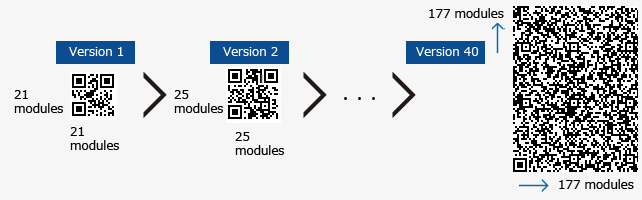
\includegraphics[width=.7\textwidth]{versionVarietyImage.png}
            \caption{On peut voir la taille de différents QR codes en fonction de leur version.\\Source : \url{https://www.qrcode.com/en/about/version.html} (consulté le 12/02/2021)}
            \label{fig:versionQR}
        \end{center}
    \end{figure}
    
    \item \textbf{Niveau de correction d'erreurs d'un QR code} : Les QR codes ont été conçus pour être résistants à la saleté ou l'usure. Cela est possible grâce à l'utilisation du "Code de Reed-Solomon", une méthode également utilisée sur les CD et DVD. Il existe 4 niveaux de correction : L (7\% de correction), M (15\%), Q (25\%) et H (30\%).\footnote{Source : \url{https://www.qrcode.com/en/about/error_correction.html} (consulté le 12/02/2021)}\\
    
    \item \textbf{Contenu d'un QR code} : Il s'agit tout simplement de l'information obtenue par l'utilisateur scannant le QR code. Nous définissons dans la partie \ref{GenQRCode} le type et la méthode d'encodage de ce contenu.\\
    
    \item \textbf{Dynamisme} : Ici le terme de dynamisme est utilisé pour décrire la logique algorithmique définissant le contenu d'un QR code suivant des paramètres (ex: temporel, valeur retournée par un appel externe, compteur...). Un QR code dynamique est donc un QR code possédant du dynamisme.\\
    
    \item \textbf{Plugin} : Dans le cadre de ce projet, un plugin désigne un programme écrit par l'exploitant lui permettant de définir le dynamisme d'un QR code.\\
    
    \item \textbf{Programme Standalone} : Un programme dédié spécifiquement à l'affichage du QR code. Celui-ci est décrit comme "Standalone" car il est capable de fonctionner par lui même (ne nécessite pas de serveur web, autres infrastructures lourdes...). L'affichage du QR code se limite donc à l'écran de la machine où le programme est exécuté.\\
    
    \item \textbf{Exploitant} : L'exploitant est la personne qui utilisera le système de QR code dynamique pour transmettre des informations aux utilisateurs (ceux qui scanneront les QR codes). Dans notre situation l'exploitant serait vraisemblablement notre client Serge Chaumette.\\
    
\subsection{Standard QR code}

Le QR code doit être bien contrasté, avec un fond clair, posséder un "zone calme" (un contour de la même couleur que le fond tout autour du QR code). La quantité maximale de données stockée est également bornée : environ 3.6 Ko \footnote{La taille maximale est la version 40, 177 * 177 positions, soit 31 329 bits ou environ 3.9 Ko, et le niveau de correction d'erreur minimal est de 7\% donc environ 3.6 Ko. La valeur réelle dépend en réalité du mode utilisé : 7 089 caractères en mode numérique, 4 296 en mode alphanumérique, 2953 caractère en mode octet et 1817 caractère en mode Kanji.}.\\

Le contenu d'un QR code est toujours une chaîne de caractères (sauf utilisation particulière). Par exemple un texte comme "Hello world" ou une URL comme "https://google.fr" sont encodés de la même manière. C'est le lecteur de QR code qui va interpréter "l'URL" comme telle. 

Pour étendre les fonctionnalités du QR code, un certain nombre de structures de contenu ont été définies au fil des années. On peut voir un liste des structures de contenu (les plus répandues) supportées par les QR codes sur la figure \ref{fig:listStructureContent}


\begin{figure}[H]
    \begin{center}
        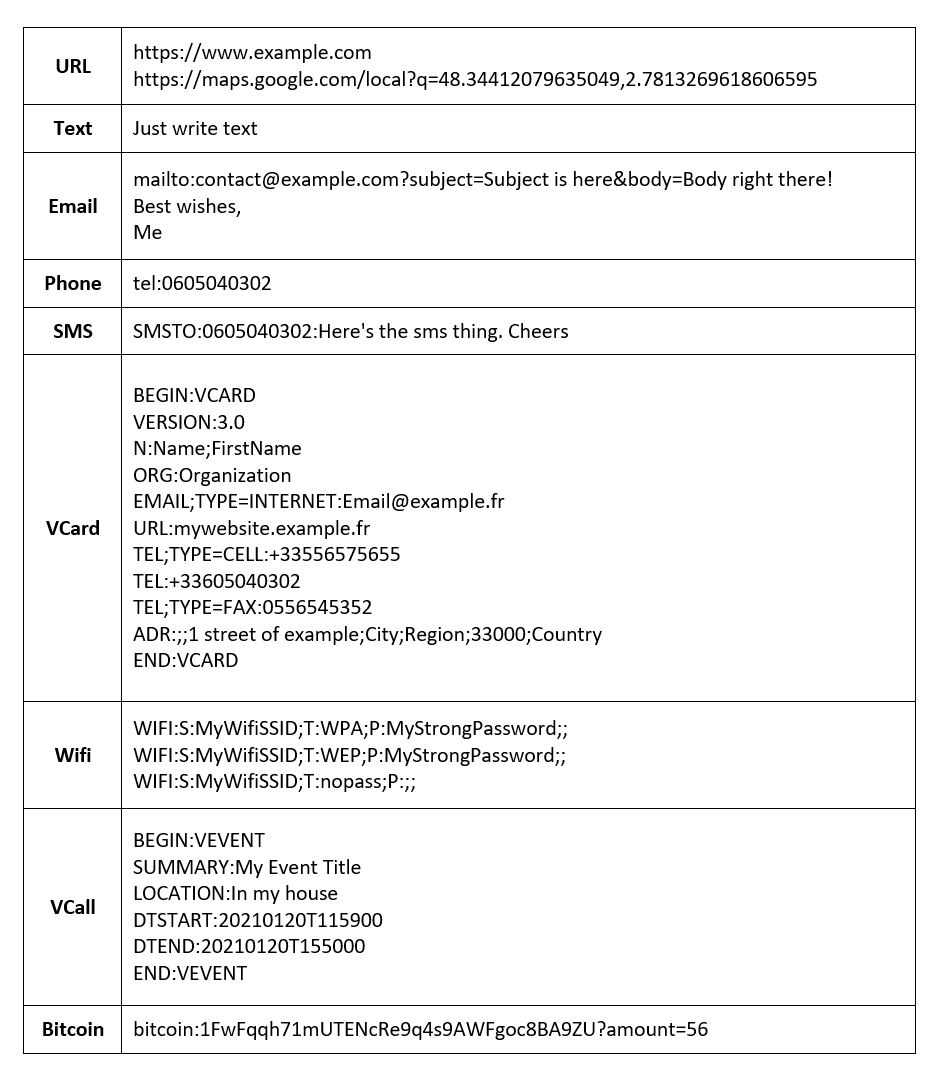
\includegraphics[width=.6\textwidth]{possible to do with QrCode.JPG}
        \caption{Liste des structures de contenu les plus répandues et supportées par les QR codes.\\Source : \url{https://github.com/zxing/zxing/wiki/Barcode-Contents} (consulté le 12/02/2021)}
        \label{fig:listStructureContent}
    \end{center}
\end{figure}


\end{itemize}

\section{Étude de l'existant}

\iffalse % Multi-line comment 
\subsection{Pseudo-code du client}

\begin{flushleft}


Nous n'avons pas d'architecture logicielle de base pour ce projet, cependant notre client nous a fourni un pseudo-code d'exemple de plugin non définitif que voici :\\

\begin{lstlisting}
---global time_slot[]=...
global phone_number[]=...

QRcodeContentGenerator(){

time = getTime()
for in in 1, max_time_slots
if (time in time_slot[i])
    return (phone_number[i], CONTENT_TYPE_PHONE_NUMBER)
}
\end{lstlisting}

Ce pseudo-code se rapproche d'un langage Python ou Java. Les deux tableaux en global contiendraient les tranches horaires et les numéros de téléphones associés à générer dans les QR codes dynamiques.\\
Notre client nous as précisé que ce plugin n'est qu'une approche de ce qu'il aimerait obtenir.

\end{flushleft}
\fi % End multi-line comment 

\subsection{Systèmes similaires aboutis}
L'idée de lier QR code et dynamisme n'est pas quelque chose de nouveau.\\
Une rapide recherche sur internet nous présente de nombreux liens présentant ou vendant ce type de service :\\

\begin{itemize}

    \item \textbf{uQR.me} (\url{https://uqr.me/qr-code-generator}):\\
    uQR.me est un service payant de création de QR code dynamique par redirection (le QR code est statique et renvoie vers un serveur de redirection web. Le dynamisme a lieu au niveau de cette page de redirection. Voir le tableau dans la partie \ref{compApproches} pour plus de détails). uQR.me semble cibler principalement les entreprises ou organisations qui souhaitent utiliser des QR codes au sein de leur campagne publicitaire. Le service propose la création en quelques clics de QR codes dynamiques pour divers usages. Le prix varie de 4,95\$ par mois pour 2 QR codes, à 49,95\$ par mois pour 1 000 QR codes. Nous suspectons que ce service ne conviendrait pas à notre client car celui-ci veut pouvoir écrire un script définissant le dynamisme des QR code dynamique (les plugins). L'interface ici se veut très accessible et il n'est pas question d'écrire des lignes de codes. Nous pensons donc que uQR.me n'est pas adapté de part sa simplicité qui est ajustée pour un usage grand public. Nous suspectons qu'aucun service en ligne ne permettra l'utilisation de scripts écrits par l'utilisateur à cause des risques d'exécution de code arbitraire\footnote{Code arbitraire est employé pour nommer une action à faire faire à une machine sans que le propriétaire soit d'accord. Plus d'info : \url{https://en.wikipedia.org/wiki/Arbitrary\_code\_execution} (consulté le 12/02/2021)}\\
    
    \item \textbf{qrd°by} (\url{https://qrd.by/#dynamic-qr-code}):\\
    qrd°by offre un service payant similaire à uQR.me. Il s'agit là encore de QR codes dynamiques par redirection, ciblant des agences de marketing et entreprises souhaitant lancer une campagne publicitaire. Plusieurs fonctionnalités sont proposées notamment la possibilité de programmer des redirections différentes suivant l'heure de la journée. Le prix de l'abonnement varie entre gratuit (1 QR code et 100 scans par jour), à 35€ par mois (500 QR code, nombre de scans illimités). Le service souffre malheureusement du même problème soulevé pour le service précédant : le client sera très vite limité par l'interface de création de QR code lorsqu'il souhaitera avoir un usage qui ne rentre pas dans les usages prédéfinis par le site.\\
    
    \item \textbf{DynQR} (\url{https://github.com/bn4t/dynamic-qr}):\\ 
    DynQR est un service web écrit par Benjamin Nater en Go. Le code source est disponible sur GitHub, sous licence GPL-3.0. DynQR se décrit comme un service web très simple et léger permettant de créer des QR codes par redirection. Il n'y a pas de page de connection, tout le monde peut créer des QR codes dynamiques. Le système ne propose qu'un type de contenu pour les QR codes : des liens URL. Également, il n'est pas possible de programmer le comportement du QR code dans le temps, la modification du contenu se fait manuellement. Ce programme ne correspond donc pas de tout au besoin de client mais pourrait tout de même être une bonne base si on implémente l'approche de dynamisme par redirection.\\
    
    \item \textbf{PHP Dynamic Qr code}\\(\url{https://github.com/giandonatoinverso/PHP-Dynamic-Qr-code}):\\
    PHP Dynamic Qr code offre un service web maintenu par Giandonato Inverso et disponible sur GitHub sous licence MIT. Il offre un service beaucoup plus complet que DynQR, se rapprochant déjà plus des services payant comme uQR.me et qrd°by. Il est possible de créer un grand nombre de QR codes type, personnaliser l'apparence du QR code, son niveau de correction d'erreur, sa taille. Il propose également un tableau de bord permettant de créer, modifier, et voir le nombre de scans pour chaque QR code. L'interface est facile à utiliser et visuellement aboutie. Une démonstration est disponible ici \url{https://www.giandonatoinverso.it/qrcode/} (consulté le 12/02/2021). Tout comme DynQR, il ne semble pas possible de programmer le dynamisme des QR codes, juste d'effectuer des modifications manuelles sur le type de redirection.
    
    \item \textbf{A.M.C. System} (\url{https://github.com/hardeepnarang10/attendance-automation}):\\
    A.M.C. System est un système d'apparence complexe, permettant de noter la présence des étudiants aux cours. Le système est développé en Python par Hardeep Narang, disponible sur GitHub sous la licence GPL-3.0. C'est un programme intéressant car notre client avait justement évoqué l'idée d'utiliser les QR codes dynamiques pour cet usage précis. Malheureusement A.M.C. System répond à ce seul besoin et donc son fonctionnement est très différent de ce que l'on souhaite pour notre projet : avec  A.M.C., c'est l'étudiant qui génère un QR code avec une application sur son smartphone et le fait scanner à l'entrée des salles de cours.
    
\end{itemize}

De manière générale, nous voyons que peut de services proposent de "programmer" le dynamisme des QR codes, seulement de le modifier manuellement. C'est un usage qui est suffisant pour la plupart des campagnes marketing (la cible numéro 1 de ces services), mais pas dans notre cas. De plus, tous ces services ne proposent que l'approche par redirection et pas par dynamisme intégré (voir le tableau dans la partie \ref{compApproches} pour plus de détails). Aucun service que nous avons trouvé ne propose la création de plugins pour définir avec beaucoup plus de contrôle.

\subsection{Bibliothèques}

Quelle que soit l’approche que nous choisissons, il sera nécessaire de générer des images de QR code. Nous avons recherché des bibliothèques permettant de simplifier la génération de QR codes sous Python et sous Java (comme expliqué dans la partie besoins, ce sont les deux langages imposés par le client).\\
Pour Python, un des premiers résultats de notre recherche était PyQRCode 1.2.1 (\url{https://pypi.org/project/PyQRCode} consulté le 12/02/2021). La bibliothèque est maintenue par Michael Nooner et est sous licence BSD. Nous avons également envisagé la bibliothèque qrcode 6.1 (\url{https://pypi.org/project/qrcode/} consulté le 12/02/2021) maintenue par Lincoln Loop, également sous licence BSD. Cependant nous avons trouvé que cette dernière avait un manque de documentation : il y a quelques exemples, mais il manque un vrai document expliquant toutes les options. PyQRCode propose ce type de documentation ici : \url{https://pythonhosted.org/PyQRCode/} (consulté le 12/02/2021). De plus PyQrCode permet de créer plus facilement les QR Codes (la plupart des QR codes peuvent être générés en 1 à deux lignes).\\

Pour Java, nous avons testé la bibliothèque ZXing 3.4.1 (\url{https://github.com/zxing/zxing} consulté le 12/02/2021) maintenue principalement par Sean Owen et distribuée sous licence Apache-2.0. Le choix de cette bibliothèque vient du fait que ZXing semble être le choix "numéro 1" pour la génération de code barre (1D et 2D) sous Java : 9/10 des premiers résultats pour "qr code java library" font référence à celle-ci. Avec recherche, nous émettons l'hypothèse que cette popularité provient du fait que ZXing est utilisé par Google pour l'analyse des code barres dans les images indexées par son moteur de recherche, mais également en tant que lecteur de code barre par défaut sous Android et dans d'autres produits Google\footnote{Source : \url{https://opensource.google/projects/zxing} (consulté le 12/02/2021)}.

\section{Scénarios}
\label{scenario}

\`A la suite de l'échange avec le client et de l'analyse des besoins, deux approches pour l'implémentation du concept de dynamisme semblent possibles :\\

\begin{itemize}
  \item \textbf{QR codes à dynamisme intégré} - Le dynamisme a lieu au niveau de l’affichage du QR code. Le QR code affiché change périodiquement.\\
  \item \textbf{QR codes à dynamisme par redirection} - Le QR code est statique et renvoie vers un serveur de redirection web. Le dynamisme a lieu au niveau de cette page de redirection.\\
\end{itemize}

\subsection{Approche utilisant des QR codes à dynamisme intégré}

\subsubsection{Liste des parties qui composent ce système}

\begin{itemize}
  \item \textbf{Plugins} - Un programme écrit par l'exploitant lui permettant de définir le dynamisme d'un QR code.\\
  
  \item \textbf{Interface} - Permet de définir la forme globale d'un plugin et de mieux séparer code client/code programme.\\
  
  \item \textbf{Fonction orchestratrice} - Prend en paramètres un plugin et un chemin. Le plugin lui fournit le contenu qu'elle transmet à la \textbf{génération de QR code}.\\
  
  \item \textbf{Génération de QR code} - Permet de créer une image PNG ou SVG du QR code à partir d'une chaîne de caractères.\\
  
  \item \textbf{Intermédiaire web} - Gère l'appel au logiciel back-end, fournit le QR code produit à la partie web.\\
  
  \item \textbf{Affichage client web} - Va demander la dernière version du QR code à fréquence régulière à l'\textbf{intermédiaire web}. C'est cette partie qui va permettre au navigateur de toujours présenter à l'utilisateur la dernière version du QR code.\\
  
  \item \textbf{Affichage standalone} - À partir d'un fichier de plugin, affiche le QR code correspondant à l'écran de l'ordinateur.\\

\end{itemize}

Voici ci-dessous un schéma permettant de montrer les interactions entre chacune des parties du systèmes et les acteurs. La chronologie des interactions est définie dans les scénarios (\ref{scen:1A} et \ref{scen:1B}).

\begin{figure}[H]
\begin{center}
  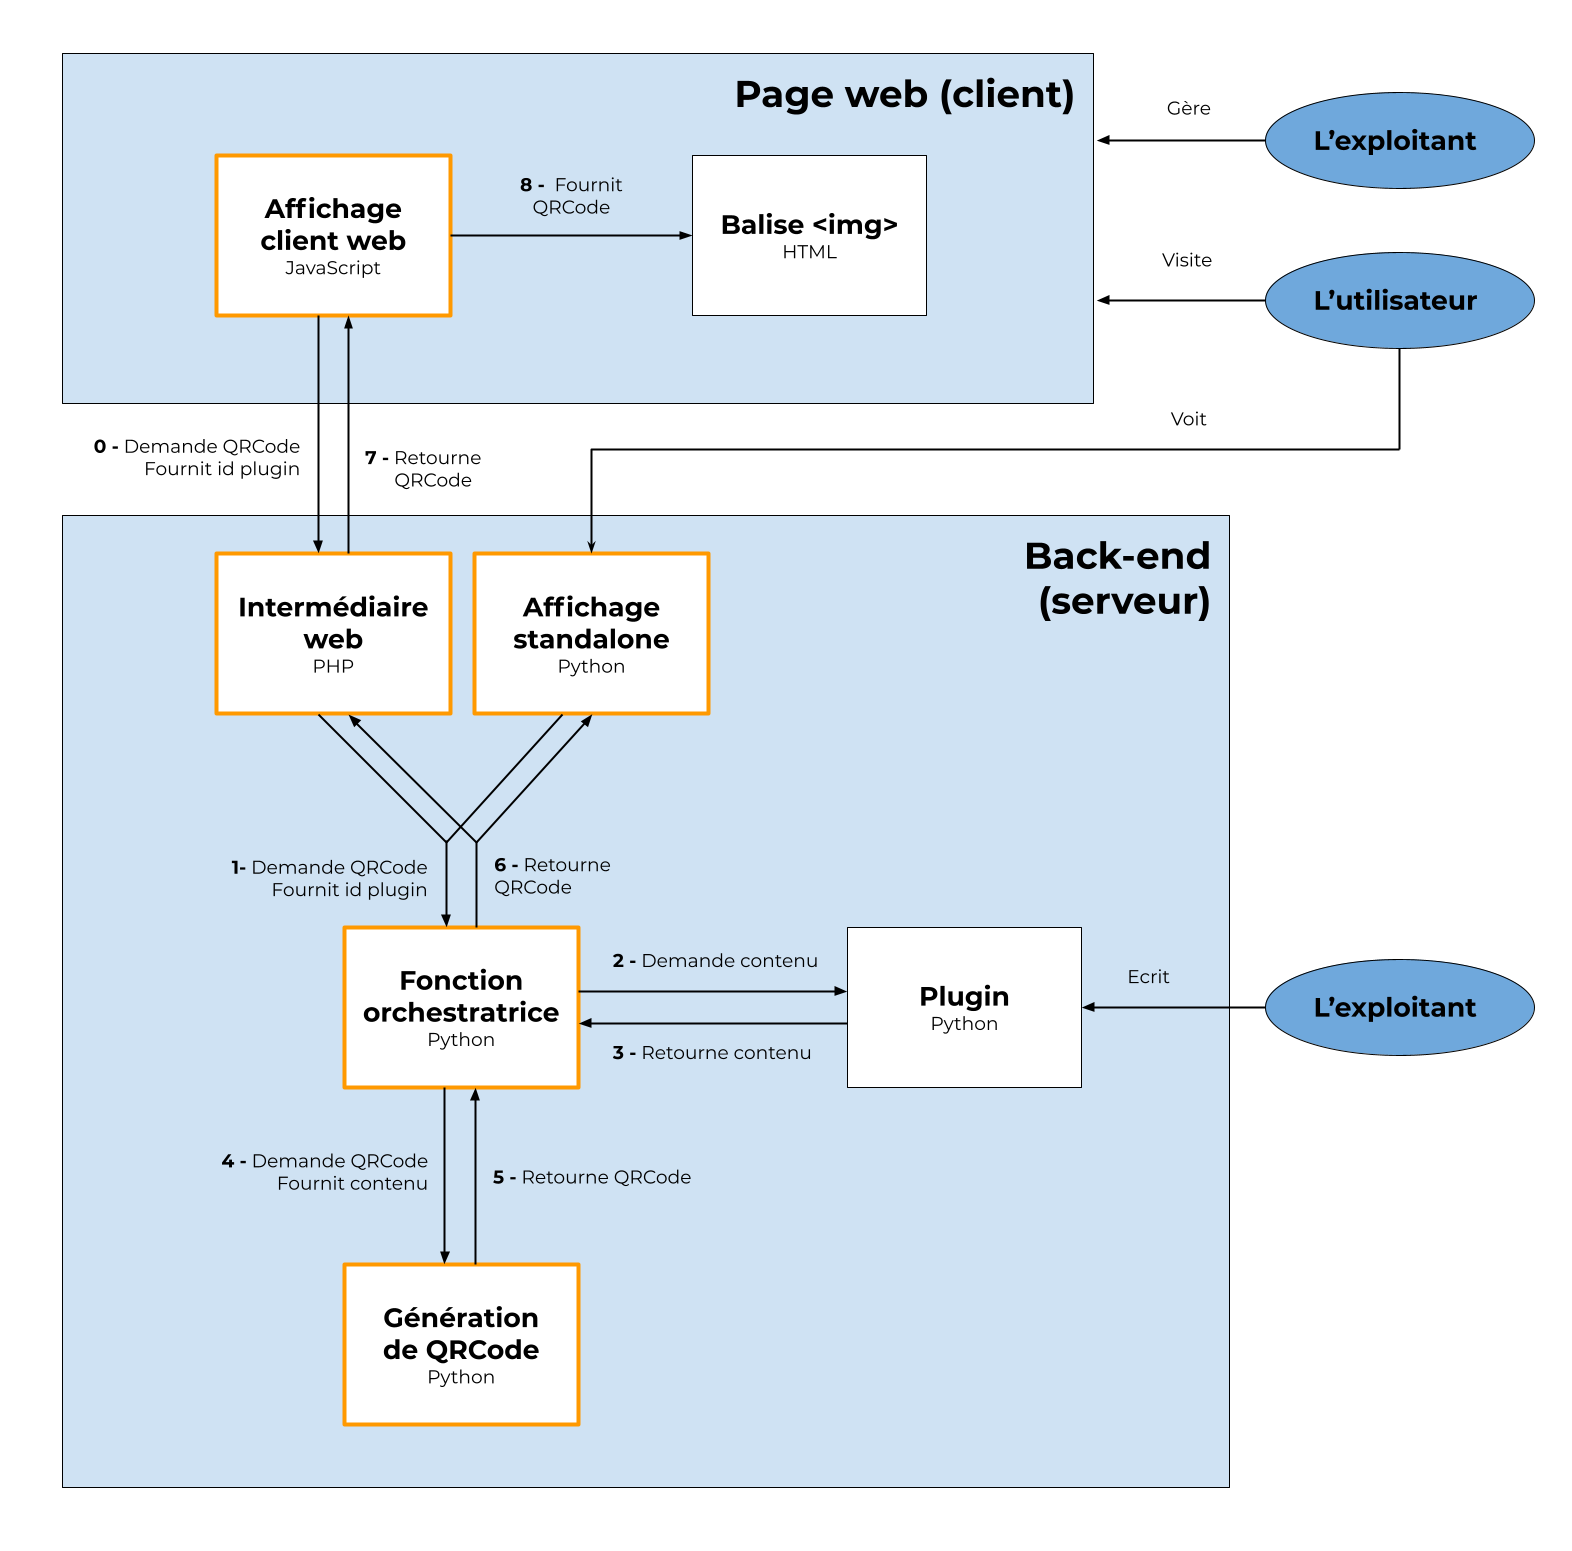
\includegraphics[width=.8\textwidth]{Organigramme QRCode.png}
  \caption{Les ellipses bleu foncé sont les acteurs : l'exploitant et l'utilisateur (qui visite la page web ou se présente devant l'écran de l'affichage standalone). Les rectangles sont les parties du système et ceux entourés en orange sont celles que nous devons coder. C'est-à-dire toutes sauf les balises <img> (qui sont à la charge de l'exploitant d'ajouter sur son site web) et les plugins (qui encore une fois sont écrits par l'exploitant).}
\end{center}
\end{figure}

\subsubsection{Scénario A : une requête web}
\label{scen:1A}

Afin de présenter comment ces différents systèmes fonctionnent ensemble, regardons l'enchaînement des évènements lorsqu'un client visite une page web contenant un QR code dynamique. Les numéros entre parenthèses correspondent aux numéros d'étapes sur le schéma ci-dessus.\\

\begin{itemize}
  
  \item Un utilisateur visite la page web.
  \item Le serveur lui fournit le code HTML, CSS, JS.
  \item Une fois la page chargée, (0) l'\textbf{Affichage client web} (fonction JS) fait une requête pour récupérer la dernière version de QR code dynamique au serveur.
  \item (1) L'\textbf{intermédiaire web} (code PHP) reçoit la demande et fait une requête à la \textbf{fonction orchestratrice} (back-end Python) pour obtenir l'image.
  \item (2) La \textbf{fonction orchestratrice} exécute le plugin passé en paramètre et (3) génère donc le contenu pour le QR code. (4) La fonction transmet ensuite le contenu à la fonction de \textbf{génération de QR code} qui produit l'image à l'emplacement souhaité.
  \item (5 et 6) De retour à l'\textbf{intermédiaire web}, (7) celui-ci retourne à l'\textbf{affichage client web} le chemin pour accéder à l'image.
  \item (8) Pour finir l'\textbf{affichage client web} modifie la balise <img> vide pour lui faire afficher l'image. Après une période de temps (qui sera définie par le plugin et transmise par l'\textbf{intermédiaire web}), l'\textbf{affichage client web} réitère l'opération et fait à nouveau une requête (retour à l'étape 1).
  
\end{itemize}

\subsubsection{Scénario B : Affichage standalone}
\label{scen:1B}

Nous pouvons constater que les parties \textbf{Plugins}, \textbf{Interface}, et \textbf{Génération de QR code} sont communes aux utilisations sur le web et en standalone. Détaillons tout de même le processus en utilisant le même schéma :\\

\begin{itemize}
  
  \item L'exploitant ouvre l'\textbf{afficheur standalone}. Celui-ci est pré-chargé avec l'ID du QR code.
  \item (1) \textbf{L'affichage standalone} fait une requête pour récupérer la dernière version de QR code dynamique au serveur.
  \item (2) La \textbf{fonction orchestratrice} exécute le plugin passé en paramètre et (3) génère donc le contenu pour le QR code. (4) La fonction transmet ensuite le contenu à la fonction de \textbf{génération de QR code} qui produit l'image à l'emplacement souhaité.
  \item (5 et 6) De retour à l'\textbf{affichage standalone}, celui-ci l'affiche à l'écran
  \item L'utilisateur se présente devant l'écran de \textbf{l'affichage standalone} et peut le scanner.\\
  
\end{itemize}


\subsection{Approche des QR codes à dynamisme par redirection}

\subsubsection{Liste des parties qui composent le système}

Un système de QR code fonctionnant par redirection dynamique implique un changement quasi-complet de l'architecture logicielle. Comme pour l'affichage standalone, seules les parties \textbf{Plugins}, \textbf{Interface}, et \textbf{Génération de QR code} restent inchangées.\\

\begin{itemize}
  \item \textbf{Plugins} - Programme écrit par l'exploitant lui permettant de définir le dynamisme du QR code.\\
  
  \item \textbf{Interface} - Permet de définir la forme globale d'un plugin et de mieux séparer code client/code programme.\\
  
  \item \textbf{Génération de QR code} - Permet de créer une image PNG ou SVG du QR code à partir d'une chaîne de caractères.\\
  
  \item \textbf{Administration web} - Permet la création et la gestion des QR codes dynamiques par le biais d'une interface web.\\
  
  \item \textbf{Serveur de redirection web} - Lorsqu'un utilisateur visite une page de ce serveur web, celui-ci obtient un contenu généré dynamiquement par les plugins. Éventuellement l'utilisateur peut être automatique redirigé vers l'application téléphone, envoi de SMS, de mail ou vers une autre page web.\\
  
\end{itemize}

Afin de présenter comment ces différents systèmes fonctionnent ensemble, regardons l'enchaînement des évènements dans trois scénarios différents (étape dans la vie d'un QR code dynamique) : A - La génération du QR code (ce qui n'implique pas la génération d'un plugin), B - La création / modification d'un plugin, et C - Le scan d'un QR code par l'utilisateur. Les numéros entre parenthèses correspondent aux numéros d'étapes sur le schéma ci-dessus.\\

\begin{figure}[H]
\begin{center}
  \noindent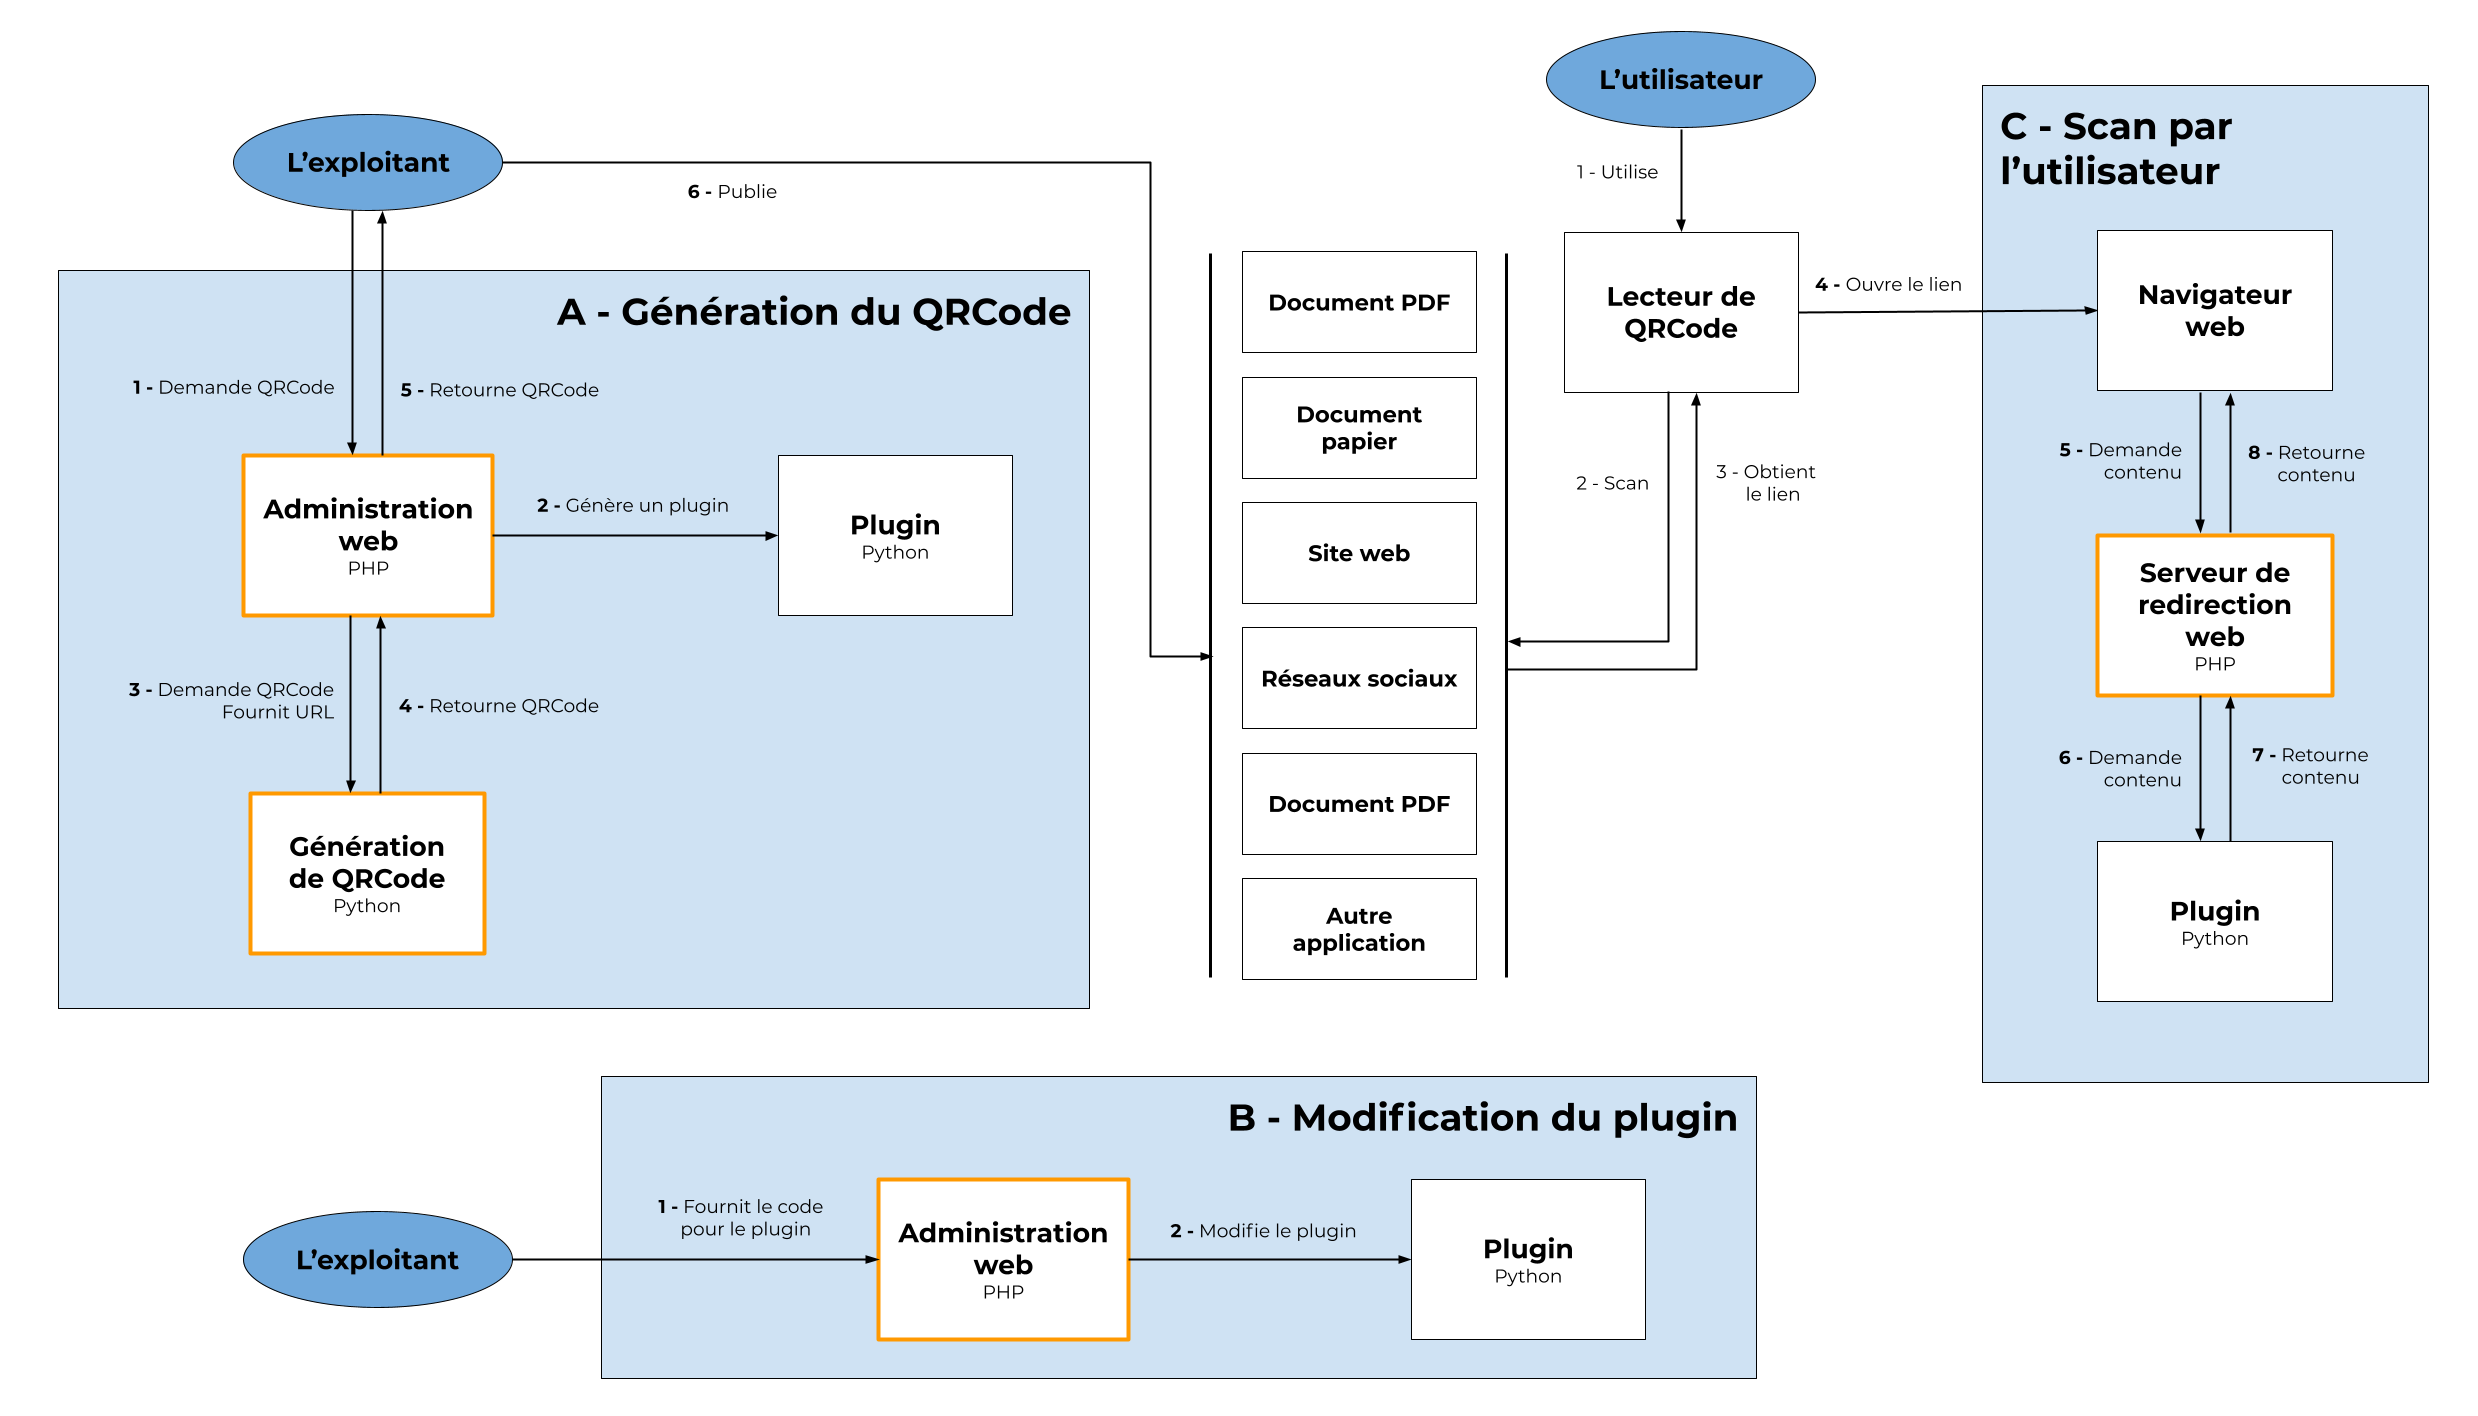
\includegraphics[width=\textwidth]{Organigramme QRCode redirection.png}
  \caption{Comme pour l'autre schéma, les ellipses bleu foncé sont les acteurs : l'exploitant et l'utilisateur. Les rectangles sont des parties sur système et ceux entourés d'orange sont celles que nous devons coder.}
\end{center}
\end{figure}


\subsubsection{Scénario A : création d'un QR code par l'exploitant}

\begin{itemize}
  
 \item L'exploitant se connecte à l'interface d'\textbf{administration web}.
 \item (1) Il appuie sur un bouton pour créer un nouveau QR code dynamique. Il peut également indiquer un titre et ou description pour le retrouver plus facilement dans le futur.
 \item L'\textbf{administration web} génère en interne un ID unique (différent des ID déjà générés).
 \item (2) Un \textbf{plugin} par défaut est généré, possédant comme nom de fichier l'ID.
 \item (3) L'\textbf{administration web} demande ensuite la création d'un QR code dont le contenu est une URL pointant vers le serveur de redirection web. L'URL possède également l'ID précédemment généré.
 \item (4 et 5) Le QR code est fournis à l'exploitant.
 \item Celui-ci peut maintenant publier le QR code, que ce soit sur internet, dans un document numérique ou papier.
  
\end{itemize}

\subsubsection{Scénario B : modification d'un plugin par l'exploitant}

A la suite du scénario A, un QR code a été crée. L'exploitant va maintenant pouvoir modifier/créer le plugin.

\begin{itemize}
  
 \item L'exploitant se connecte à l'interface d'\textbf{administration web}.
 \item L'exploitant peut voir la liste des ID/QR code généré, avec la date de création, le titre, description.
 \item En cliquant sur le bouton modifier d'un des QR code, une interface apparaît
 \item Sur cette page l'exploitant peut modifier le code du plugin ainsi que le faire tourner pour vérifier sa valeur actuelle
 \item (1) Une fois terminé, il peut sauvegarder les modifications.
 \item (2) Le \textbf{plugin} est modifié pour prendre en compte les modifications.
  
\end{itemize}

\subsubsection{Scénario C : scan d'un QR code par un utilisateur}

\begin{itemize}
  
 \item Un utilisateur trouve un QR code généré par l'exploitant.
 \item (1) Il le scanne ce qui (2) ouvre un lien web pointant vers le \textbf{serveur de redirection web}.
 \item L'URL possédant également l'ID du QR code, le \textbf{serveur de redirection web} le récupère est l'utilise pour (3) demander un contenu dynamique au \textbf{plugin} correspondant. (5) Celui-ci lui retourne le contenu. (6) Suivant le type du contenu, le \textbf{serveur de redirection web} peut rediriger l'utilisateur vers une autre page web, lancer l'application téléphone, mail ou SMS, ou simplement afficher du texte ou une image
  
\end{itemize}

\iffalse % Multi-line comment 
\begin{flushleft}
Dans cette partie nous devrons justifier nos choix de conception par rapport aux besoins fonctionnels puis non fonctionnels du client.\\
Par exemple on retrouvera ici le comparatif des langages testés, une mise en opposition des contraintes/avantages avec des schémas/diagrammes/stats pour expliquer pourquoi python et pas java (ou l'inverse).\\

Cela sert donc à introduire la partie 4 Choix de conception.\\

OU ALORS --> on fusionne avec la partie 4 dans laquelle on explique mieux nos choix.
\end{flushleft}
\fi % End multi-line comment 


\subsection{Comparaison des deux approches}
\label{compApproches}

\noindent Voici ci-dessous un tableau pour présenter les principales différences entre les deux approches :\\

    \noindent\begin{longtable}{ | m{.475\textwidth} | m{.475\textwidth} | } 
    \hline
    \textbf{Dynamisme intégré} & \textbf{Dynamisme par redirection} \\ 
    \hline
    Le dynamisme a lieu au niveau de l’affichage du QR code. Le QR code affiché change périodiquement. & Le QR code est statique et renvoie vers un serveur de redirection web. Le dynamisme à lieu au niveau de cette page de redirection.\\
    \hline
    Le QR code ne peut être affiché que sur une interface qui a été prévu pour : le(s) site(s) web de l'exploitant tournant sous PHP et l'afficheur standalone. Un travail de développement doit être effectué pour chaque nouveau système sur lequel le QR code doit être intégré. & Le QR code est statique, il peut donc être exporté, inclus dans un document, imprimé, publié sur n'importe quel site : ce n'est qu'une image. Pas besoin de créer un afficheur standalone.\\
    \hline
    L'intégration d'un QR code dynamique sur un site web nécessite que le système et le serveur web soit sur la même machine. Il faut également inclure un fichier PHP accessible depuis internet, ainsi qu'un script JavaScript sur chaque page possédant un QR code. & Le système est complètement séparé de tout autre systèmes (un serveur web PHP est tout de même nécessaire mais il n'a pas de rapport avec le serveur web du site sur lequel le QR code est déposé).\\
    \hline
    Le contenu est limité à 3,9 Ko (peut être contourné en utilisant un lien web). & Le contenu n'étant pas sur le QR code, il n'y a pas de limite fixe sur la taille du contenu. Cela pourrait être une vidéo de 1.6 Go par exemple, un livre, un jeu...\\
    \hline
    Vis-à-vis des QR codes limité dans le temps (le contenu devient inaccessible à un horodatage spécifié), le contenu dont on souhaite contrôler l'accès se trouvant dans le QR code, n'importe qui peut le copier, le prendre en photo, le publie ailleurs. Il est donc très facile de contourner ce système. & Le contenu dont on souhaite contrôler l'accès étant sur la page web de destination du QR code, l'exploitant a un contrôle totale sur la disponibilité de cette page. Il peut à chaque instant la bloquer, ou la débloquer à souhait.\\
    \hline
    Il n'est pas possible de mettre un mot de passe pour l'accès à l'information & La page pourrait demander à l'utilisateur d'entrer un mot de passe pour accéder à l'information.\\
    \hline
    Un nouveau QR code doit être généré à chaque changement de son contenu & Un seul QR code est généré.\\
    \hline
    Il n'est pas possible de savoir par qui, quand et où le QR code à été scanné. & Il serait possible de connaître les adresses IP, l'heure et la position (si on imprime plusieurs QR code à différents endroits d'un bâtiment par exemple) des personnes scannant le QR code. On pourrait également noté les informations du client web comme l'OS, la version du navigateur, la résolution de l'écran...\\
    \hline
    Pas besoin de serveur web pour l'affichage standalone & Nécessite un serveur web quelque soit l'utilisation \\ 
    \hline
    Il y a 6 parties qui composent cette approche. & Il y a 4 parties qui composent cette approche, et elles sont plus indépendantes les unes des autres. De manière générale, cette approche est moins complexe à mettre en oeuvre.\\
    \hline
    L'utilisateur qui scanne n'as pas besoin d'un accès internet pour accéder au contenu (sauf si il s'agit d'un lien web) &  L'utilisateur doit avoir un accès internet (ou au moins une connection au réseau local sur lequel tourne le serveur web)\\ 
    \hline
    Aucune charge réseau pour l'affichage standalone, charge réseau supérieur pour l'utilisation web car l'image du QR code est plus lourde que son contenu seul. & Charge réseau proportionelle au nombre d'utilisateurs\\
    \hline
    \end{longtable}

\bigskip
L'approche par redirection a été exclue par le client dans le cadre initial du projet car elle requiert une installation plus lourde (hébergement d'un service web, ouverture de port, potentielle utilisation de bases de données...). De ce que l'on a compris, le client possédant déjà un serveur web tournant sur PHP, toutes ses "difficultés" sont en réalité inexistantes. Comme vu dans le tableau comparatif ci-dessus, l'installation, l'utilisation et surtout l'intégration des QR codes serait fortement simplifié. De manière générale, les deux approches sont compatibles avec les besoins fonctionnels imposés par le client, mais chacun possède des avantages et inconvénients. L'inconvénient majeur du système par redirection est que l'utilisateur final doit avoir un accès internet.


\section{Besoins}

\begin{flushleft}
Les besoins fonctionnels seront classés dans l'ordre de priorité d'implémentation qui nous semble cohérent.\\
Niveau 1 : priorité élevée.\\
Niveau 2 : priorité intermédiaire.\\
Niveau 3 : priorité faible.
\end{flushleft}

\subsection{Besoins fonctionnels}


\subsubsection{Génération}

\begin{itemize}

  \item \textbf{Générer des QR} : Niveau 1\\
  \label{GenQRCode}
  Les QR codes permettent l'utilisation de nombreuses structures de données/fonctionnalités, nous souhaitons ici avoir au minimum : le lien URL, le numéro de téléphone et le message textuel. Plusieurs contraintes s'imposent : pour l'encodage du contenu, nous allons nous limiter à ceux nativement compatibles avec le standard QR code, à savoir la norme ASCII étendue et le Shift JIS (caractères japonais). Pour la longueur du contenu, la quantité d'information maximale est de 3,9 Ko (soit 4 296 caractères alphanumérique).\\
  
  Les QR codes seront exporté au format PNG : la taille des images étant petite et de type bitmap (les pixels sont soit blanc), l'utilisation d'autres formats comme JPEG ou SVG ne serait pas adapté. Par exemple une image de QR code version 40, résolution 1000x1000 pixels au format PNG pèse 5.54 Ko, là où le même QR code exporté au format JPEG pèse 377 Ko !\footnote{La différence peut être expliqué en partie par le fait que le PNG supporte le mode bitmap, là ou JPEG doit utilisé le mode RGB. Le mode bitmap utilise 1 bit par pixel là où le mode RGB utilise un octet par canal par pixel (soit 24 bits par pixel).}. De plus, le PNG propose une compression sans perte ce qui est préférable pour faciliter le scan du QR code.\\
  
  Risques/Parades : Le contenu du QR code généré ne correspond pas au contenu donné en paramètre.\\
  Tests : Il faudra vérifier la prise en charge de toutes les fonctionnalités en générant des QR codes puis en vérifiant leur contenu après scannage. Cela pourra être testé de manière automatique grâce à un générateur de QR codes qui s'auto-évalue.\\

  \item \textbf{Configurer la génération des QR codes par le biais de plugins} : Niveau 1\\
  Les plugins sont des programme écrit par l'exploitant lui permettant de définir le dynamisme du QR code. Ces programmes devront suivre une forme définit par une interface que nous écrirons\footnote{Nous n'avons pas encore mis au point sur interface mais nous pouvons imaginer que les plugins posséderons une fonction qui retournera un objet possédant un attribut \textbf{content} (un string). Nous listerons d'autres attributs possibles dans la partie \ref{ExtensionsProposées}}.\\
  
\end{itemize}

\subsubsection{Affichage / intégration}

\begin{itemize}
  
  \item \textbf{Rafraîchir le QR code affiché à l'écran} : Niveau 1\\
  Dans le cas de l'approche par dynamisme intégré, la méthode d'affichage doit permettre de rafraîchir le QR code présenté à période régulière. Ce rafraîchissement doit se faire de manière automatique. Pour une utilisation standalone (en local sur l'ordinateur de l'exploitant), il suffit de réexecuter le plugin, générer l'image de QR code et la recharger dans le programme d'affichage. Pour une utilisation web, ce rafraîchissement nécessite d'avoir un code tournant sur l'ordinateur client. Nous utiliserons un court script écrit en JavaScript pour cela.\\
  
  \item \textbf{Afficher le QR code dynamique dans un programme standalone} : Niveau 1\\
  Comme indiqué dans le besoin précédant, le programme standalone est un programme qui tourne en local sur l'ordinateur de l'exploitant. Nous pouvons bien sûr imaginer que le moniteur en question est un téléviseur positionné à l'entrée d'un magasin ou d'un bureau (voir les exemples d'utilisations présentés dans l'introduction).\\

  \item \textbf{Intégrer le QR code dynamique sur le site web de l'exploitant} : Niveau 2\\
  Le site web de l'exploitant tourne sous PHP (ou du moins accepte l'utilisation de code PHP). Dans le cas de l'approche par dynamisme intégré, cela pose une contrainte sur le langage à utiliser pour le dialogue entre le page web et le back-end. Il sera nécéssaire de vérifier la compatibilité avec les différents navigateurs web.\\
  
  \item \textbf{Imprimer les QR codes} : Niveau 3\\
  Ce n'est pas un besoin indiqué par le client. Cependant nous avons juger utile d'en parler pour mieux définir la avantage et inconvénient de chaque approche. De part la nature des QR code à dynamisme intégré, il n'est pas possible de les imprimer : il faut un code machine pour modifier le QR code affiché. Ce n'est pas un problème avec le QR code à dynamisme par redirection qui n'est qu'une simple image statique pointant vers une URL. Il existe seulement une contrainte majeure : \textbf{le smartphone de l'utilisateur scannant le QR code doit avoir accès à internet.}\\
  
  \item \textbf{Intégrer un QR code sur n'importe quel site web} : Niveau 3\\
  De même que le besoin précédent, ce n'est pas un besoin indiqué par le client. Pour une utilisation sur le web, l'approche par dynamisme intégré nécessite de déposer du code PHP et JS pour gérer le rafraîchissement des QR codes. Cela restreint leurs utilisations aux sites web dont on est administrateur : il n’est pas possible de les publier sur les réseaux sociaux et autres. Également, bien que PHP soit massivement utilisé sur les serveurs d’hébergement web, ils existent d’autres frameworks tel que Asp .Net, Enyo, Ruby on Rails, NodeJs... Pour intégrer les QR codes sur un site utilisant une autre technologie que PHP, il serait nécessaire de réécrire une nouvelle version de l’intermédiaire web.
  Encore une fois, ce n'est pas un problème avec le QR code à dynamisme par redirection.\\
  
\end{itemize}

\subsubsection{Autres fonctionnalités}

\begin{itemize}
  
  \item \textbf{Donner une limite temporelle au QR code} : Niveau 2\\
  Il doit être possible d'indiquer un horodatage auquel le QR code n'est plus visible, ou renvoie un message tel que "Le contenu n'est plus disponible". C'est ici que l'approche part dynamisme intégré a ces limites : dans l’éventualité où un utilisateur télécharge l’image, la prend en photo ou potentiellement la publie, il n’est pas possible d’empêcher quiconque de scanner et de visionner le contenu du QR code. L'approche par redirection permet un réel contrôle d'accès au contenu. Cette différence s'explique par le fait que dans la première approche, le contenu dont on souhaite limiter l'accès se trouve dans le QR code, là où le système par redirection ne fournis que l'URL pour y accéder.\\
  
\end{itemize}

\subsection{Besoins utilisateurs non fonctionnels}

Avant de commencer cette partie, nous souhaitons indiqué que l'exploitant à posé comme condition que le langage utilisé pour la création des plugins soit Python ou Java. C'est pour cela que vous constaterez une dualité entre les deux (et ces deux là seulement) dans les besoins suivants. Nous terminerons par le besoin \textbf{"langages utilisé pour l'écriture des plugins"} qui servira de conclusion aux observations faîtes dans les autres besoins.\\

\begin{itemize}
  
  \item \textbf{Performances} :\\
  Trois aspects peuvent impacter les performances de notre système : le temps de réponse, la vitesse d'exécution et la mémoire utilisées. Nous n'avons définit aucune contrainte avec le client. Nous allons donc nous même nous fixer des contraintes réalistes en supposant que le système tourne sur du matériel informatique standard\footnote{En opposition avec un serveur de calculs dédiée. Les tests ayant était effectué sur un de nos ordinateurs personnels c'est cela que l'on considère "du matériel informatique standard". La configuration du PC était un Ryzen 5 2600 (6 coeurs, 12 threads) avec 8 Go de mémoire vive DDR4.}, que d'autres programmes peuvent également être en fonctionnement (on pense notamment à un serveur web).\\
  
  \iffalse
  
  Quelle que soit l'approche que nous choisissons, il sera nécessaire de générer des images de QR code. Nous avons fait des tests permettant de vérifier le temps de calcul pour la génération de QR code sous Python et sous Java.
  \paragraph{}Sous Python, nous avons utilisé PyQrCode. Il s'agit d'un module permettant de manipuler plus facilement des Qr Code. (La plupart des Qr Code peuvent être générés en 2 lignes).\\
  Sous Java, nous avons utilisé la librairie Zxing (ou Zebra Crossing). Elle permet de générer des codes barres en multi-format (1 à 2 dimensions). Dans notre cas, nous nous sommes intéressés au format à 2 dimensions (celle d'un code-barre). \\
  
  \fi
  
  Pour notre premier test, nous avons générer des QR codes de taille 500x500 pixels avec un niveau de correction L et de version "auto" (cela signifie que la bibliothèque sélectionne la version de QR code de taille minimal où la quantité de donnée fournit peut être stocké). Le contenu était "Ceci est un test de QRCode numéro i" où i varie avec l'indice du QR code en cours de génération. Nous avons générer des lots de quantité différente (1, 5, 10 , ...). Nous avons choisi ces propriété car cela correspond à des cas d'utilisation habituelle. Vous pouvez retrouver les algorithmes utilisés dans l'annexe à la fin du document. Voici les résultats ci-dessous :

    \begin{figure}[H]
        \centering
        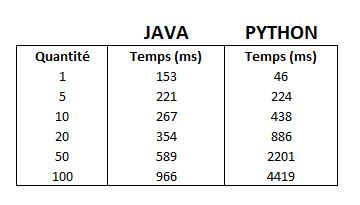
\includegraphics[width=.5\textwidth]{vitesse small.JPG}
        \caption{On peut voir que Python est presque 3 fois plus rapide pour produire 1 QR code. Cependant, le temps de calcul croit linéairement avec le nombre de QR code pour Python, là où Java semble croire de manière logarithmique.}
    \end{figure}
 
  Nous avons fais un second test avec des QR codes "extrême" : niveau de correction H (la plus élevée), version 40 (la plus grande), et une résolution de 1000x1000 pixels. Le contenu reste inchangé ainsi que les algorithmes utilisées. Voici les résultats : 
  
  
      \begin{figure}[H]
        \centering
        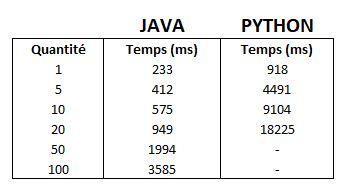
\includegraphics[width=.5\textwidth]{vitesse big.JPG}
        \caption{On peut voir que Python est presque 4 fois plus lent que Java. Et cet écart ne fait que croître avec la quantité. Java est ici le gagnant incontesté.}
    \end{figure}

    
  Il faut cependant prendre en compte deux paramètres pour correctement interpréter ses résultats vis-à-vis de ce projet : même en générant des QR code extrême (le pire scénario possible), il est possible de générer 1 QR code à la seconde. Au vu de l'utilisation demandé pour ce projet, ces résultats nous paraissent satisfaisant quel que soit le langage choisi.\\
  
  Vis-à-vis de la mémoire vive, la machine virtuel Java (JRE) consomme 20 Mo à vide (une boucle while sans opération). Lors de la génération de 500 QR codes sur 16 secondes, la consommation est resté parfaitement constante à environ 300 Mo de mémoire vive utilisée. Python lui à une consommation à vide de 10 Mo, et de 15 Mo lors de la génération des QR codes (suivant le même protocole). Python est donc meilleurs pour une consommation mémoire faible.\\
  
  Vis-à-vis de la taille des fichiers produits, la différence est faible : Java produit des fichiers de 6.5 Ko et Python 5.5 Ko pour des images PNG de QR code version 40 et de taille 1000x1000 pixels. Dans tous les cas, ce sont des poids très faible, similaire à celui d'une favicon (le logo d'une page web, souvant affiché dans dans l'onglet à côté du titre de la page).\\
  
  Vis-à-vis du temps de réponse, nous avons essayé de mesure le temps qu'il faut pour afficher un "Hello world" dans les deux langages. Nous avons mesuré 0.55s pour Java et 0.59 pour Python (moyenne basé sur 10 mesures pour chaque). Nous n'avons pas de garantie mais nous pensons que ces temps prennent en compte l'inclusion des bibliothèques. Dans tous les cas ces résultats ne permettent pas de désigner un langage plus performant.\\
  
  Au delà du langage de programmation/bibliothèque utilisé, d'autres questions de performance se posent, notamment si ce système est utilisé au sein d'un site web ayant de nombreux visiteurs en parallèle. Nous avons détaillé ce point dans la \textbf{Partie 5} en expliquant pourquoi des systèmes de caches peuvent réduire considérablement la charge du système.\\

  \item \textbf{Facilité d'utilisation} :\\
  La facilité d'utilisation est un point important pour l'exploitant : il souhaite avoir le moins de code à écrire, c'est-à-dire, se limiter à l'écriture des plugins et possiblement lors de l'installation/configuration initial du système. L'écriture des plugins doit elle aussi être facilitée : nous avons pensé qu'il serait intéressant d'inclure un certain nombre de modèles types. Par exemple, une classe qui permettrait de créer un QR code pour l'envoi de mail (avec des attributs pour la boite de destination, un sujet par défaut, un corps par défaut).\\
  
  Il s'agit de fournir à l'exploitant un "formulaire de création" sous la forme d'attributs de classe. Dans un premier temps nous pourrions créer des classes "formulaire" pour les types \textbf{Text}, \textbf{URL} et \textbf{Phone}, puis d'étendre l'idée aux autres types.\\
  
  Il existe tout de même un risque : en voulant trop simplifier l'écriture des plugins, on risque de limiter les possibilités. Afin de s'assurer que notre démarche est bonne, il faudra demander des idées de plugins au client et vérifier qu'il est facile de les implémenter. Nous devrons vérifier que nos outils d'aide à l'écriture de code n'empêche pas l'écriture de système plus complexe : trouver le juste milieu entre facilité d'écriture et possibilités algorithmiques.\\

  \item \textbf{Fiabilité, sécurité} :\\
  Il est également important de limiter le risque d'erreur : un plugin (code du l'exploitant) ne doit pas pouvoir faire planter le système. Il faudra être capable de mettre en place des section de code non-modifiables par les plugins, par exemple au moyen d'interface, et/ou de classes et objets privés. C'est-à-dire, limiter la capacité des plugins à leur stricte minimum : des fonctions qui génère des chaînes de caractère.\\
  
  Vis-à-vis de la fiabilité du système, nous allons bien sûr mettre en place les tests unitaires nécessaires. Le point que nous considérons comme le plus important est de garantir la conformité du contenu du QR code selon ce que le plugin a fourni. Avec les quatre modes d'encodage du QR code, qui possèdent tous des limitations sur les plages ASCII/Unicode compatibles, un problème d'encodage est vite arrivé. Le problème devient encore plus important dans l'éventualité où nous offrons une fonctionnalité pour insérer un logo ou un court texte au centre du QR code. Afin de garantir cette conformité, nous proposons de systématiquement vérifier à l'aide d'un décodeur les QR codes générés en comparant le contenu donnée en entrée et obtenu en sortie.\\
  
  Ici, le choix du langage a également sont importance. Java possède des mots-clés puissant comme final ou private, ainsi qu'un typage fort. Python lui propose plutôt des manières pour indiquer que des attributs sont privées, sans réelles protections. Au moyen de techniques comme la "décoration de nom" ou Name mangling\footnote{Source : \url{https://en.wikipedia.org/wiki/Name_mangling} (consulté le 12/02/2021)} en anglais, il est possible d'accéder et même de modifier des attributs "privées".
  Le langage Java parait donc le plus approprié pour limiter les capacités d'un plugin à "casser" le système.\\
  
  \item \textbf{Portabilité} : L'installation ou la réinstallation du système doit être rigoureusement documentée. Si possible il doit pouvoir être installé sur Windows ou Linux. Nous ne pourrons pas tester toutes les versions de Windows, et encore moins toutes les branches de Linux. Nous allons donc nous focaliser dans un premier temps sur un système tournant sur Debian 10. Nous verrons plus tard s'il est facile de porter notre système sur une machine tournant sous Windows 10. Nous avons tout de même de bon espoir en terme de portabilité de part l'utilisation de Python qui est un langage interprété, ou bien de Java. \\
  Contraintes : Multiplateforme, simple d'installation.\\
  
  \item \textbf{Le langages utilisé pour l'écriture des plugins} :\\
  Le client souhaite que les plugins soit écrient dans un langage de programmation avec lequel il est familier : Python ou Java.
  Il nous a donc fallu dégager les avantages/inconvénients des deux langages pour déterminer le plus adapté. Nous avons en premier pensé au temps de génération des QR code cependant nos faibles exigences en terme de performance ne permettent pas de déterminer un langage vainqueur (voir le besoin \textbf{Performances} ci-dessus).\\
  
  Nous nous sommes donc penchés sur le sujet de la facilité d'utilisation, que ce soit pour l'exploitant et nous mêmes. Ici Python se démarque par sa simplicité de code (voir la différence de la taille des programmes de tests en annexe), et le fait qu'il s'agisse d'un langage interprété (l'exploitant n'a pas à compilé ses plugins avant utilisation). Encore une fois vous trouverez plus de détail ci-dessus, dans la partie \textbf{Facilité d'utilisation}.\\
  
  Nous avons également étudié la question de la sécurité : quel langage permet de limiter les conséquences d'un plugin présentant des bugs ? Notre analyse montre que Java permet de mieux protéger son code à l'aide de mot-clé puissant, de son typage fort et de l'utilisation d'un compilateur qui vérifie des erreurs typiques comme une faute de frappe dans le nom d'une variable. Python ne permet que de fournir des indications sur l'utilisation des attributs d'une classe. Malgré tout, nous pensons que l'utilisation de Python ne poserait pas de réel danger dans la mesure où les plugins ont uniquement accès au pointeur de l'objet de retour de sa fonction getContent(). Cela signifie que l'exploitant ne pourra pas modifier de fonctions/objets utilisés dans le code des autres parties du systèmes. Voir le besoin \textbf{Fiabilité, sécurité} ci-dessus pour plus de détails.\\
  
  Pour finir, nous nous sommes intéressé au évolution futures. Cette fois Python (ou plutôt sa bibliothèque PyQRcode) se démarque grâce aux nombreuses options de personnalisation du QR code proposé, comme par exemple la couleur du fond, la couleur des modules, ou encore la possibilité d'exporter l'image en mode vectorielle.\\
  
  Nous avons donc décider de choisir Python comme langage pour l'écriture des plugins, et par extension la majorité du système (l'unicité du langage permet de simplifier le dialogue entre les différentes parties du programme).\\
  
\end{itemize}

\newpage
\section{Systèmes de caches}

Avec les approches simplistes proposées dans les scénarios (partie \ref{scenario}), nous pouvons imaginer qu'un site web accueillant des milliers d'utilisateurs en parallèle n'aurait pas la puissance de calcul nécessaire pour constamment générer des QR codes à la volée (de plus que la majorité du temps, leurs contenus resteront inchangés). Nous devons donc mettre en place un système de cache.


\begin{figure}[H]
    \centering
    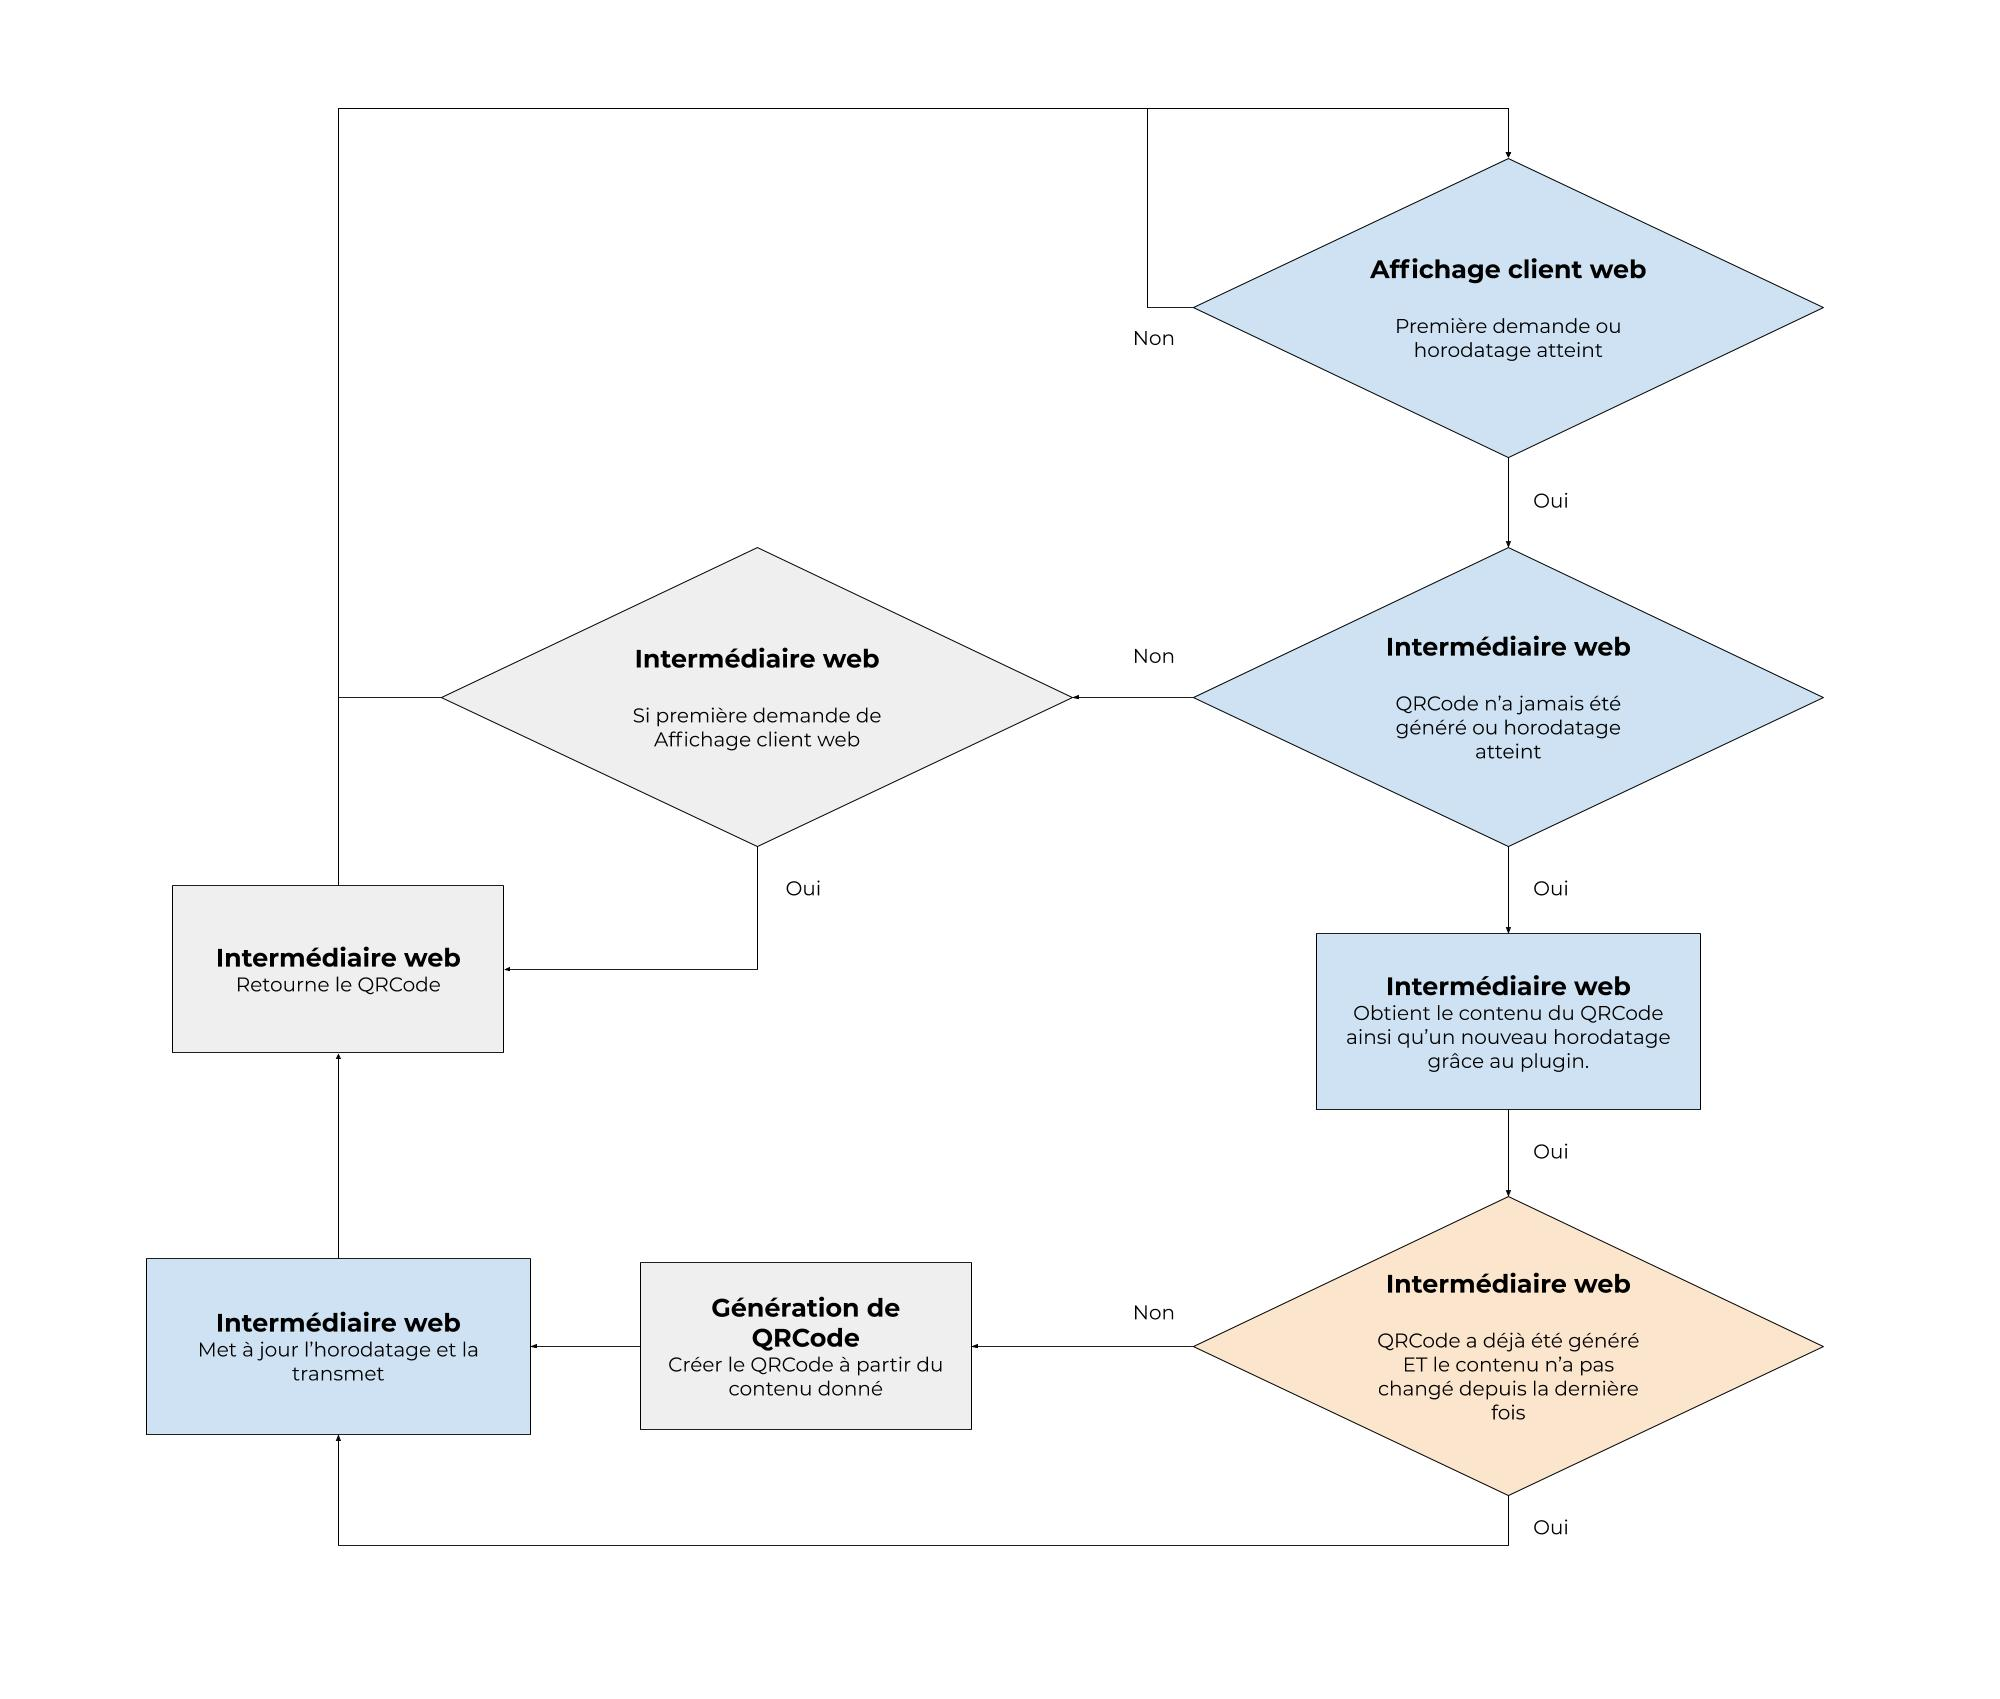
\includegraphics[width=.8\textwidth]{Logique cache.jpg}
    \caption{Diagramme logique présentant comment l'utilisation de systèmes de cache par horodatage et par hash pourrait réduire le nombre d'appel vers les plugins et la partie \textbf{Génération de QR code}. Ces deux systèmes sont expliqué de manière plus détaillé ci-dessous.}
\end{figure}

Deux systèmes pourront coexister :\\

\begin{itemize}

  \item \textbf{Cache temporel (bleu)} : les plugins devront définir un horodatage. C'est-à-dire qu'en plus de fournir le contenu à mettre dans le QR code, le plugin doit indiquer à quelle heure le contenu du QR code sera périmé. C'est généralement possible de calculer cette date, cependant, si le plugin utilise une logique plus complexe, asynchrone, ou aléatoire, il peut être impossible de connaître cet horodatage. \`A la place, le plugin peut fournir un intervalle de rafraîchissement désiré (ex : 20 secondes, 5 minutes, 1 heure...). Le système calculera directement l'horodatage à partir de l'heure actuelle et de l'intervalle. Cette méthode n'est pas sans rappeler les entêtes "Expires" utilisés en HTTP\footnote{Les entêtes "Expires" sont utilisés pour indiquer au navigateur du client que la ressource envoyée restera valide jusqu'à une certaine date. Cela évite notamment de constamment demander le même fichier de police de caractère, le même logo en haut de la page, les même feuilles de style CSS; qui sont toutes des ressources extrêmement statiques. Plus d'info : \url{https://developer.mozilla.org/en-US/docs/Web/HTTP/Headers/Expires}}. Cet horodatage pourra être utilisé par l'\textbf{intermédiaire web} et l'\textbf{Affichage client web} pour limiter les demandes de calcul et de génération des QR codes, les deux opérations lourdes de ce système.\\
  
  \item \textbf{Cache par hachage (orange)} : il est également possible de réduire d'avantage le nombre d'appels vers la fonction de \textbf{génération de QR code}. En effet, la \textbf{fonction orchestratrice} pourrait stocker le hash du contenu d'un QR code. Si après appel du plugin le hash du contenu et le même que le contenu précédent, il n'est pas nécessaire de régénérer le même QR code.\\
  
\end{itemize}

\iffalse
\section{Limitations anticipées}

\begin{itemize}

  \item Vis-à-vis des QR codes limités dans le temps, l'implémentation proposée permet uniquement de retirer l'image de l'écran (utilisation standalone) ou de la téléverser au client (utilisation dans un site web). Dans l'éventualité où un utilisateur télécharge l'image, la prend en photo ou potentiellement la publie, il n'est pas possible d'empêcher quiconque de scanner et de visionner le contenu du QR code.\\
  
  \item Pour une utilisation web, il est nécessaire de déposer du code PHP et JS pour gérer le dynamisme des QR codes. Cela restreint leurs utilisations aux sites web dont on est administrateur : il n'est pas possible de les publier sur les réseaux sociaux et autres. Pour une utilisation standalone, il est bien sûr impossible de les imprimer, ou de les intégrer à un document PDF, PowerPoint, Word...\\
  
  \item Bien que PHP soit massivement utilisé sur les serveurs d'hébergement web, il existe d'autres frameworks tel que Asp .Net, Enyo, Ruby on Rails, NodeJs... Pour intégrer les QR codes sur un site utilisant une autre technologie que PHP, il serait nécessaire de réécrire une nouvelle version de l'\textbf{intermédiaire web}. Cela dit, son code est extrêmement simple, il ne fait que passer l'information entre le front-end et back-end.\\
  
\end{itemize}

\newpage
\fi



\section{Extensions proposées}
\label{ExtensionsProposées}

\begin{flushleft}
Il s'agit ici de lister un certain nombre de fonctionnalités supplémentaires qui dépassent le cadre du sujet donnée par le client. Ils ne rentrent donc pas dans la liste des besoins. L'objectif étant de répondre dans un premier temps aux demandes du client (satisfaire le cahier des besoins), et dans un second temps de nous intéresser à l'ajout de ces extensions.\\
\end{flushleft}

\begin{itemize}

    \item Pour les QR codes limités dans le temps, pouvoir afficher la "date de péremption" (au centre ou en dessous).\\
    
    \item Pouvoir personnaliser le style visuel du QR code :
    \begin{itemize}
        \item Changer la couleur de fond et couleur du QR code.
        \item Ajouter un texte quelconque en dessous du QR code.
        \item Ajouter une icône au centre du QR code.\\
    \end{itemize}
    
    \item Le codage des caractères compatibles avec le standard QR code sont l'ASCII étendu et Shift JIS (caractères japonais). L'inclusion de l'UTF-8 semble possible par le biais du mode d'écriture binaire que propose le QR code. Cela pourrait permettre d'étendre ce système à d'autre pays, langues et systèmes d'écriture (et les emojis !).\\
    
    \item Avoir un service tournant en tâche de fond qui rafraîchit de lui même la dernière version disponible du QR code. Sans l'utilisation d'un tel service, un utilisateur web pourrait devoir attendre la première fois qu'un QR code est généré, ou est régénéré après être arrivé à la fin de son horodatage.\\
    
    \item Remplacer le système de plugins par une interface graphique permettant de paramétrer le dynamisme d'un QR code. Cela permettrait notamment de sécuriser le système : l'exécution de code arbitraire\footnote{Code arbitraire est employé pour nommer une action à faire faire à une machine sans que le propriétaire soit d'accord. Plus d'info : \url{https://en.wikipedia.org/wiki/Arbitrary\_code\_execution} (consulté le 12/02/2021)} est une faille importante dans l'éventualité où les plugins sont fournis par une personne tierce.\\
    
    \item Dans le cas des QR codes sur internet, cliquer sur l'image de QR code devrait permettre de simuler l'acte de la scanner. C'est-à-dire que cliquer sur un QR code textuel devrait faire apparaître un boite de dialogue avec son contenu, un lien devrait nous rediriger...\\
    
    \item En couplant l'implémentation du dynamisme par redirection avec une interface de paramétrage web, nous pourrions aborder l'idée de créer un service web permettant à des utilisateurs de créer un compte, créer/modifier des QR codes dynamiques, et les exporter. Nous pourrions par la suite imaginer différentes fonctionnalités comme par exemple de comptabiliser le nombre de fois que le QR code a été scanné.
  
\end{itemize}

\section{Diagramme de Gantt}

N'ayant pas eu de retour de notre client (au delà de la première séance de présentation du sujet), nous nous retrouvons dans la situation où deux approches nous semble réalisable. Les deux répondent aux besoins émis par le client, chacune ayant des avantages et inconvénients.\\

Nous avons donc décidé de suivre le planning suivi : nous allons commencer par développer les parties qui sont en commun entre les deux approches, dans l'espoir d'un retour de notre client d'ici là. Dans le cas où nous n'avons pas de retour, nous nous focaliserons sur l'approche par dynamisme intégré. La raison est que cette approche correspond mieux à la description que le client nous avait été faites d'un tel système. Lorsque l'implémentation de cette approche sera presque terminée, nous commencerons à travailler sur l'approche par redirection avec l'espoir de la finir pour le rendu final.\\ 

\noindent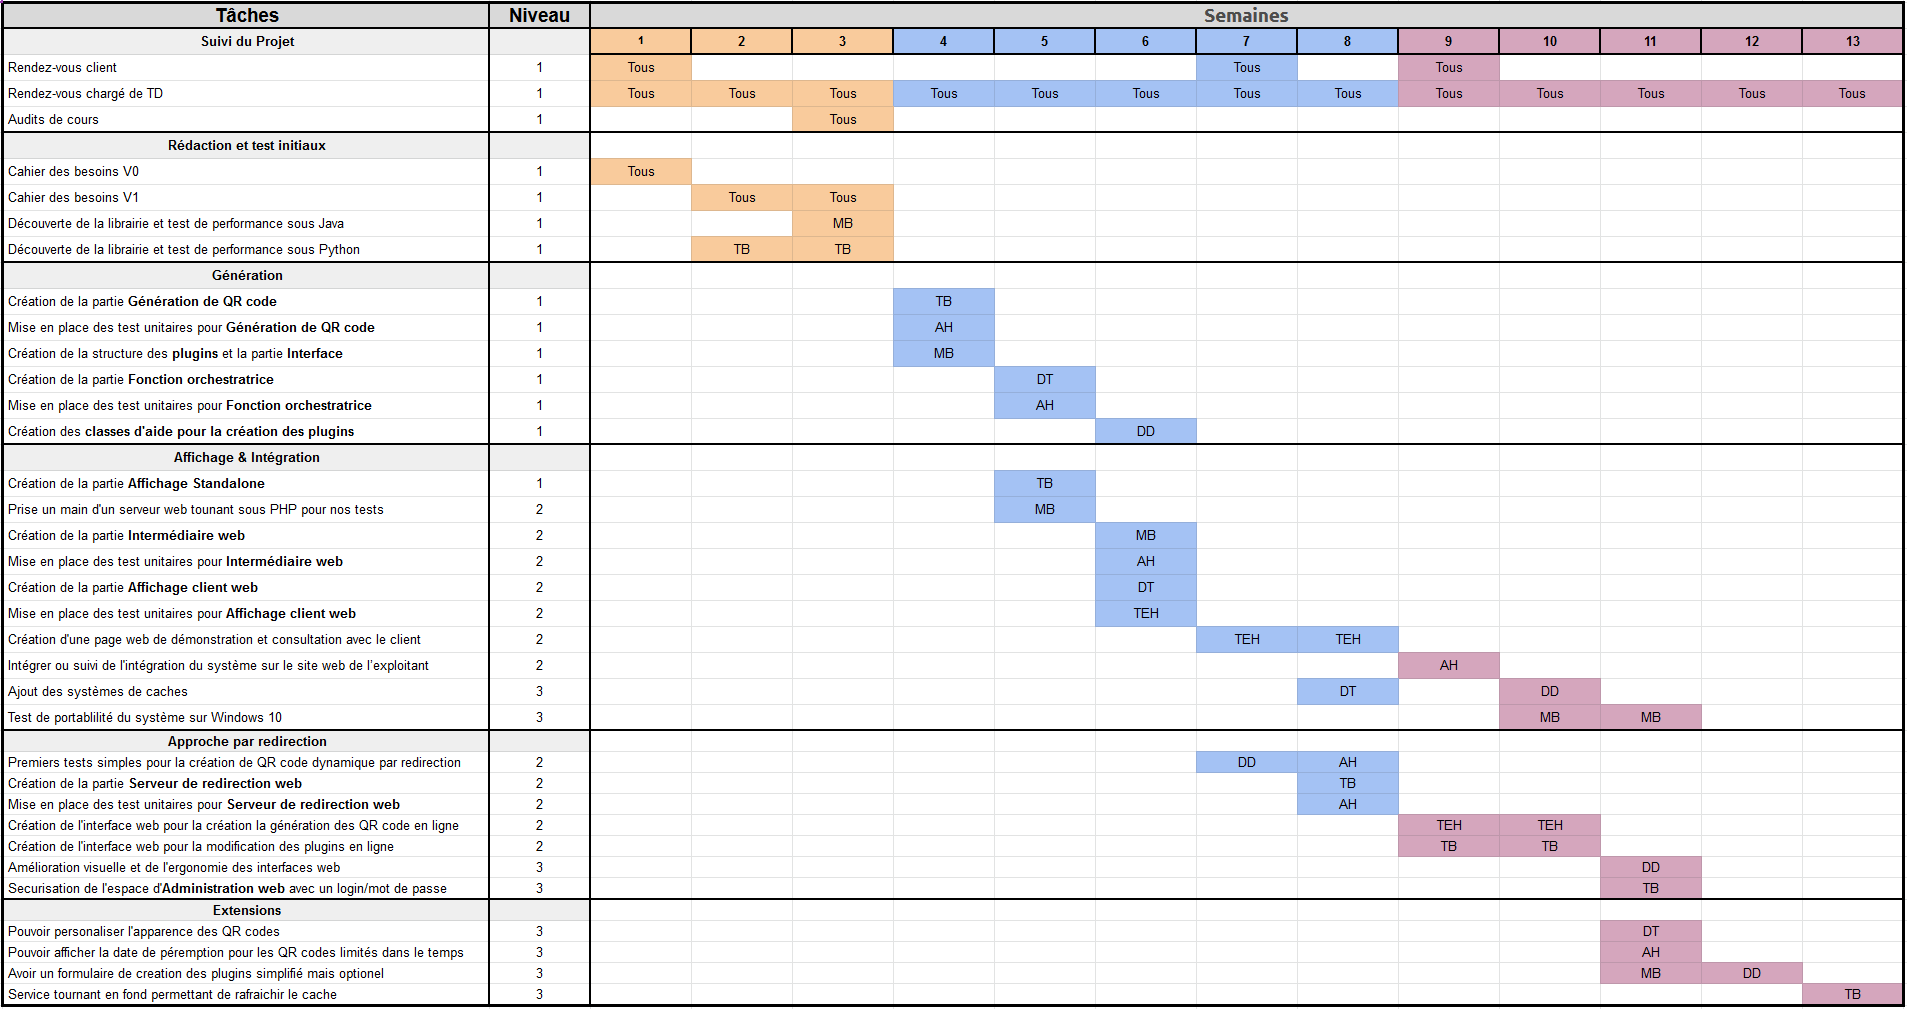
\includegraphics[width=\textwidth]{gantt.png}

\newpage

\section{Bibliographie}

\begin{itemize}

\item International Standard ISO/IEC 18004
Information technology — Automatic identification and data capture techniques — Bar code symbology — QR code\\
Disponible ici : \url{https://swisseduc.ch/informatik/theoretische\_informatik/qr\_codes/docs/qr\_standard.pdf} (consulté le 12/02/2021) \\

\item GitHub. 2021. bn4t/dynamic-qr. [site web] Disponible à : <https://github.com/bn4t/dynamic-qr> (consulté le 12/02/2021).\\
\item Burcea, C., 2021. Generating Barcodes and QR Codes in Java | Baeldung. [online] Baeldung. Available at: <https://www.baeldung.com/java-generating-barcodes-qr-codes> (consulté le 12/02/2021).\\
\item Uqr.me. 2021. Dynamic QR Code Generator - Free, custom, tracking, with logo. [site web] Disponible à : <https://uqr.me/qr-code-generator> (consulté le 12/02/2021).\\
\item GitHub. 2021. giandonatoinverso/PHP-Dynamic-Qr-code. [site web] Disponible à : <https://github.com/giandonatoinverso/PHP-Dynamic-Qr-code> (consulté le 12/02/2021).\\
\item GitHub. 2021. hardeepnarang10/attendance-automation. [site web] Disponible à : <https://github.com/hardeepnarang10/attendance-automation> (consulté le 12/02/2021).\\
\item PyPI. 2021. PyQRCode. [site web] Disponible à : <https://pypi.org/project/PyQRCode> (consulté le 12/02/2021).\\
\item Qrd.by. 2021. QR Code Generator - Create Free QR Codes. [site web] Disponible à : <https://qrd.by/#dynamic-qr-code> (consulté le 12/02/2021).\\
\item PyPI. 2021. qrcode. [site web] Disponible à : <https://pypi.org/project/qrcode> (consulté le 12/02/2021).\\
\item PyPI. 2021. zbar. [site web] Disponible à : <https://pypi.org/project/zbar> (consulté le 12/02/2021).\\
\item GitHub. 2021. zxing/zxing. [site web] Disponible à : <https://github.com/zxing/zxing> (consulté le 12/02/2021).\\



\iffalse

\item \url{https://uqr.me/qr-code-generator}\\
\item \url{https://qrd.by/#dynamic-qr-code}\\
\item \url{https://github.com/bn4t/dynamic-qr}\\
\item \url{https://github.com/giandonatoinverso/PHP-Dynamic-Qr-code}\\
\item \url{https://github.com/hardeepnarang10/attendance-automation}\\
\item \url{https://www.baeldung.com/java-generating-barcodes-qr-codes}\\
\item \url{https://pypi.org/project/qrcode}\\
\item \url{https://pypi.org/project/PyQRCode}\\
\item \url{https://github.com/zxing/zxing}\\
\item \url{https://pypi.org/project/zbar}\\

\fi


\end{itemize}

\newpage
\section{Annexe}

\subsection{Code du test de performance sous Java}
Ci dessous le code utilisé pour nos tests comparatifs entre les performances de Java et de Python pour la génération des QR codes.

\noindent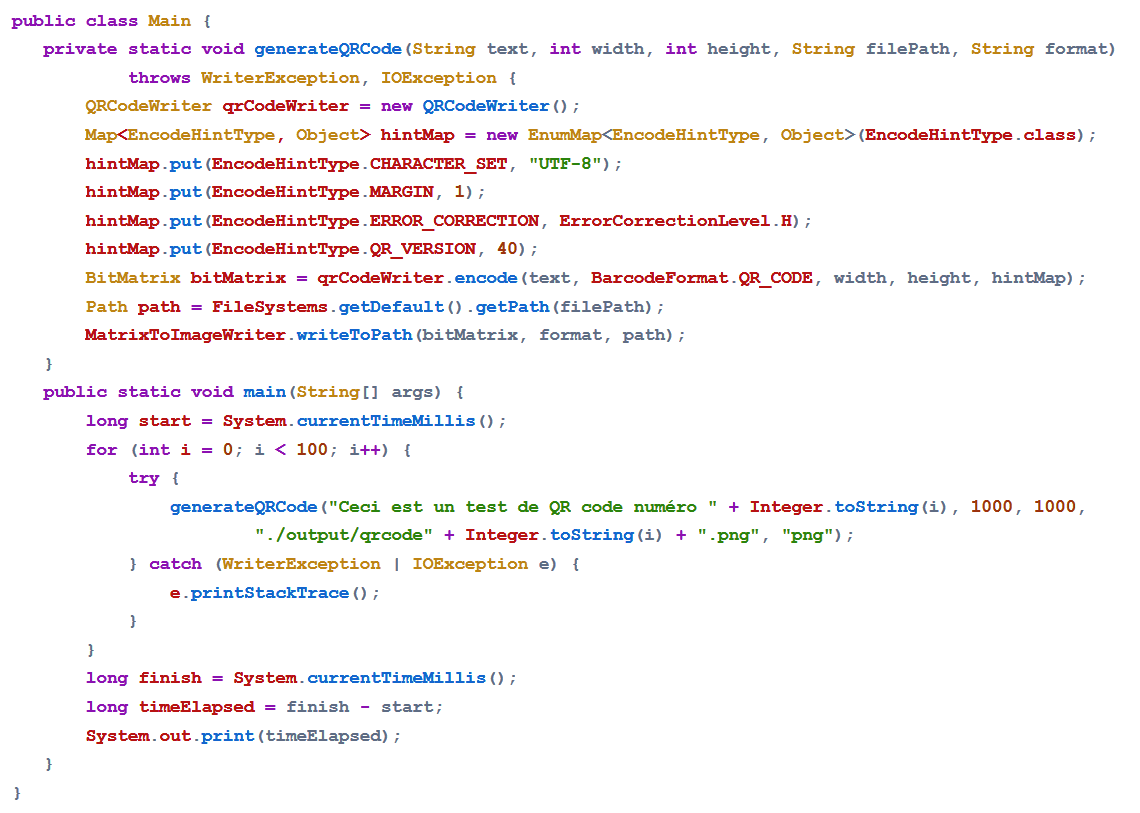
\includegraphics[width=\textwidth]{code-java.png}

\newpage
\subsection{Code du test de performance sous Python}
Un code beaucoup plus court pour le même algorithme. Veuillez ne pas prêter attention au nombre d'itération qui est différente dans les deux programmes, nous les avons testé pour différent nombre d'itération et il ne s'agit ici que de la dernière valeur entrée avant de faire une capture du code.
On peut également noter qu'il n'y a pas de méthode pour indiquer directement la taille de l'image finale. Nous pouvons la faire varier avec le paramètre "scale" qui définit la taille de chaque module.\\
La taille en pixels peut être calculée avec la formule suivante : ((version - 1) * 4 + 21) * scale.\\

\noindent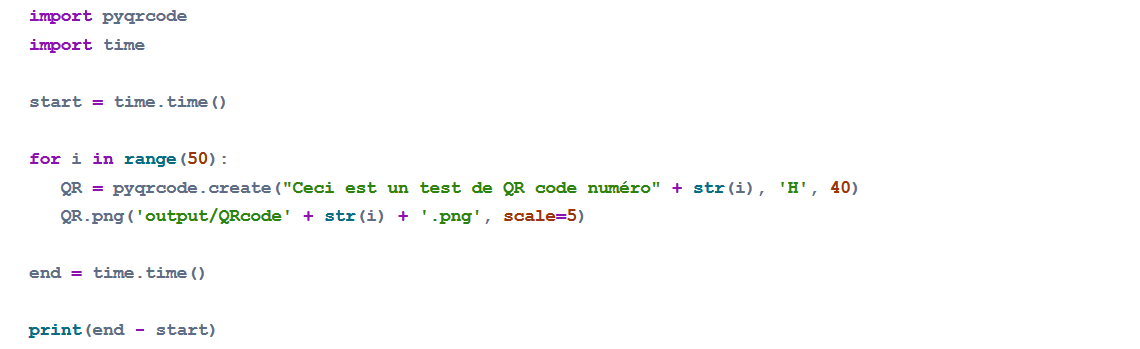
\includegraphics[width=\textwidth]{code-python.png}

\end{document}
